\chapter{Resultados}

En este capítulo se van a mostrar resultados obtenidos con las siguientes funcionalidades implementadas: Filtrado, segmentación y documentación.

Para realizar las pruebas se han utilizado la esculturas de Inmaculada Concepción y San Juan Evangelista (Figura \ref{fig:resultados/esculturas}), ambas patrimonio de la Universidad de Granada y cuyos datos DICOM han sido proporcionados por el proyecto de Portal Virtual de Patrimonio de las Universidades Andaluzas, coordinado por la Universidad de Granada.

\begin{figure}[H]
	\centering
	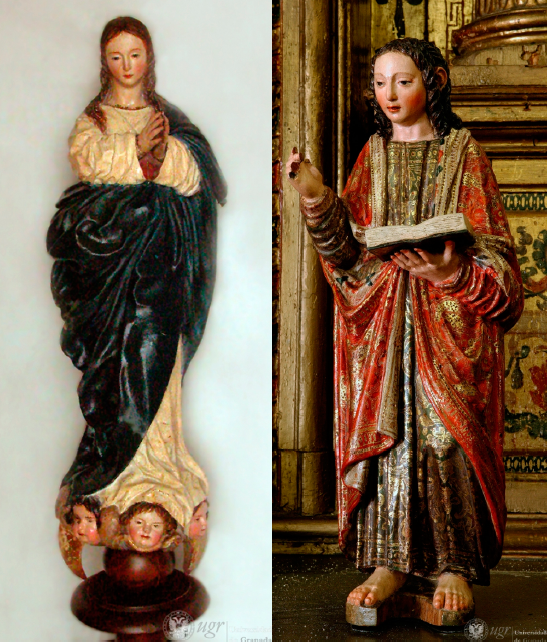
\includegraphics[width=7cm]{imagenes/resultados/esculturas}
	\caption{Esculturas utilizadas para realizar las pruebas. Inmaculada Concepción (izquierda) y San Juan Evangelista (derecha)}
	\label{fig:resultados/esculturas}
\end{figure}

\section{Filtrado}

Se implementaron los filtros de reducción de ruido \textit{gaussiano}, media y mediana dando la posibilidad al usuario a elegir ciertos parámetros.

Para probar estos filtros se ha utilizado la escultura de San Juan Evangelista que es la que más ruido presentaba.

\subsection{Filtro \textit{gaussiano}}

El filtro \textit{gaussiano} es uno de los filtros de suavizado más utilizados. A continuación se va a mostrar los resultados obtenidos con éste para 1, 2 y 3 repeticiones (Figura \ref{fig:resultados/filtrado/gaussiano}).

\begin{figure}[H]
	\centering
	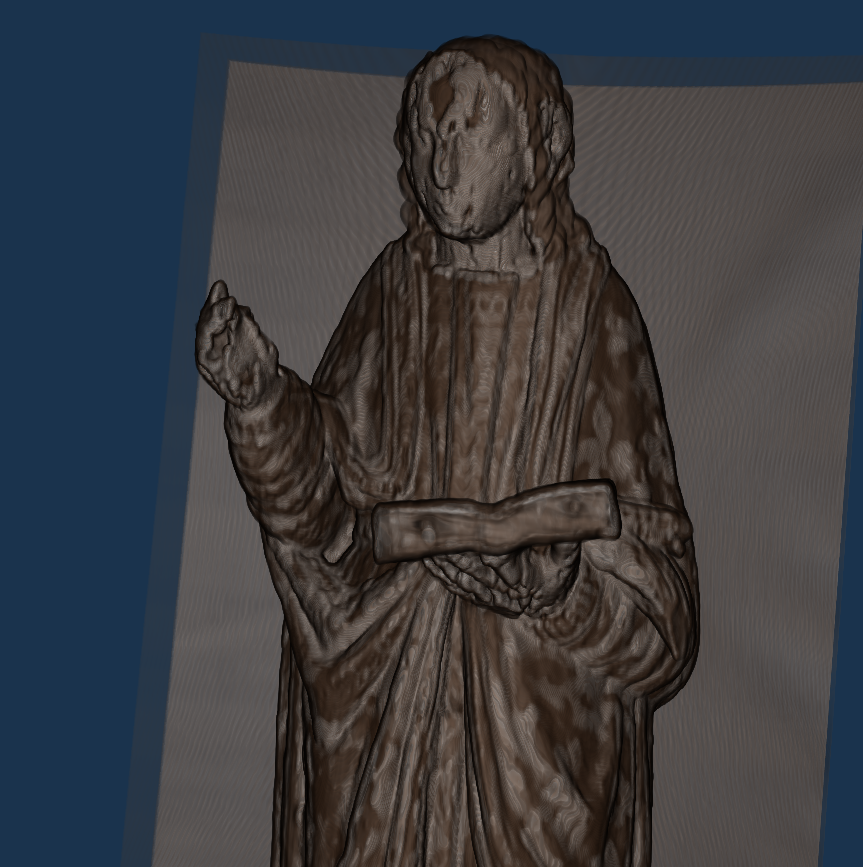
\includegraphics[width=6cm]{imagenes/resultados/filtrado/original}
	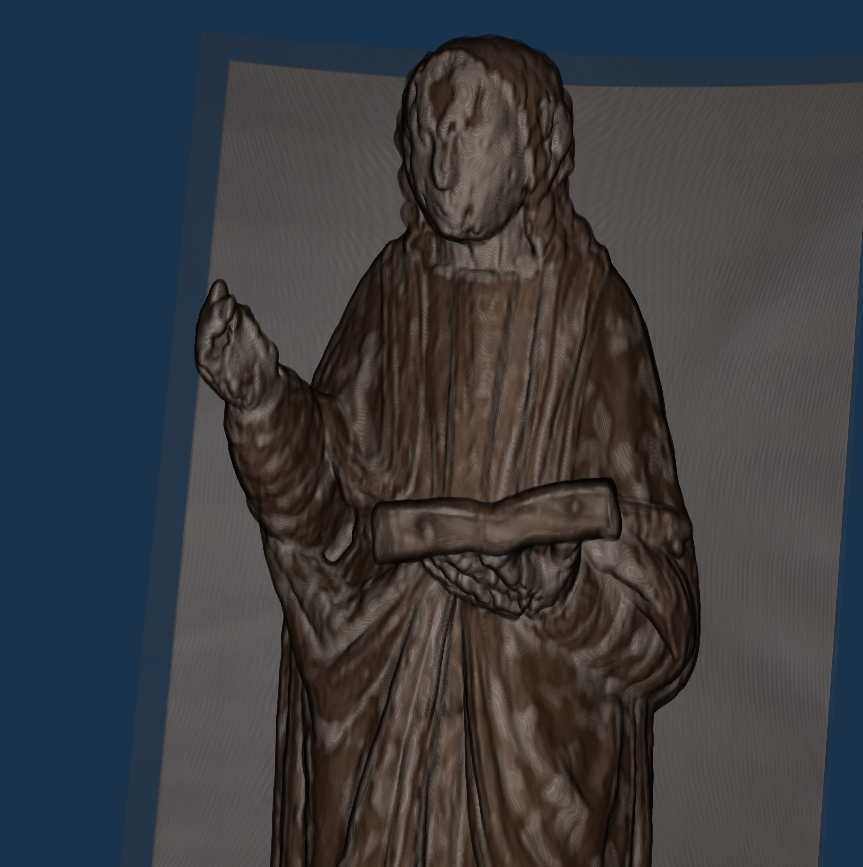
\includegraphics[width=6cm]{imagenes/resultados/filtrado/gaussiano-1}
	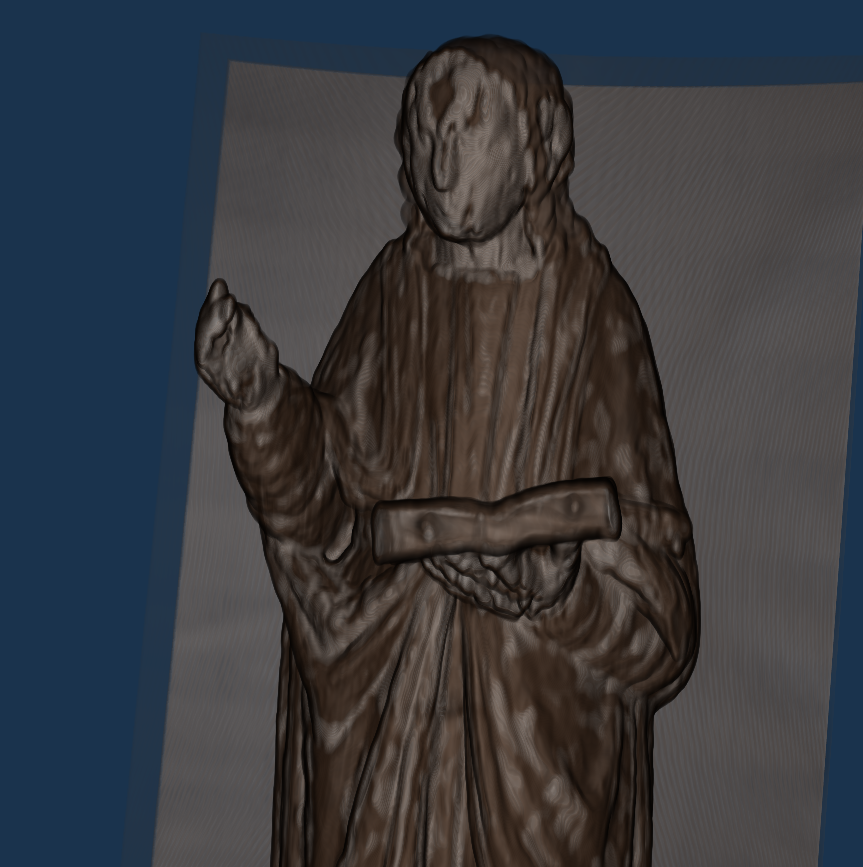
\includegraphics[width=6cm]{imagenes/resultados/filtrado/gaussiano-2}
	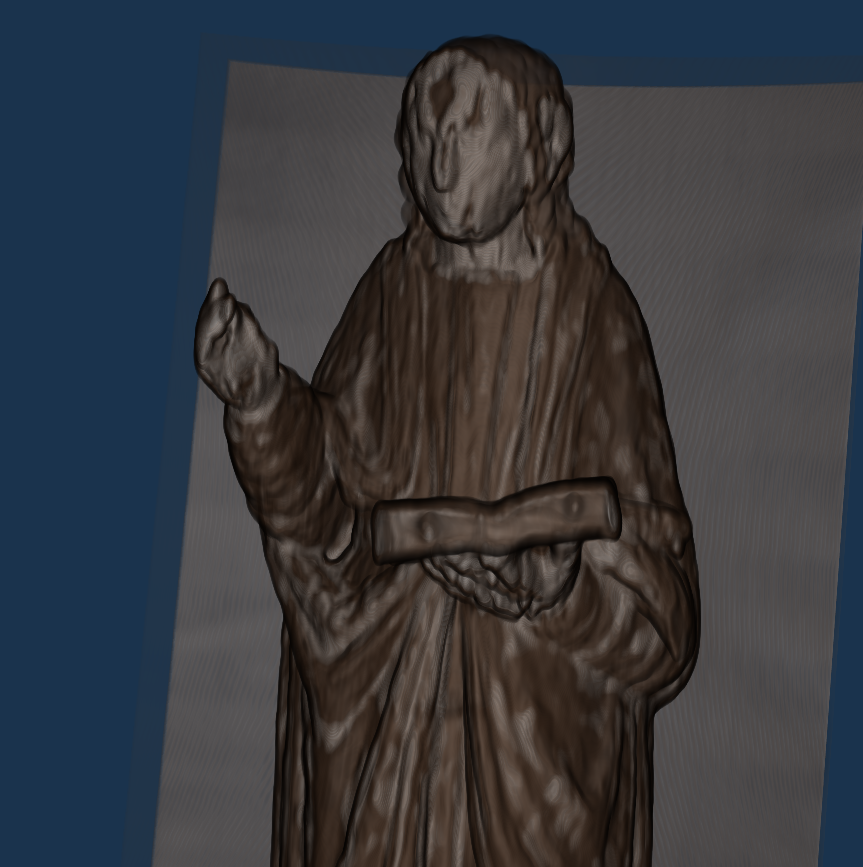
\includegraphics[width=6cm]{imagenes/resultados/filtrado/gaussiano-3}
	\caption{De izquierda a derecha y arriba a abajo: figura original y aplicando el filtro \textit{gaussiano} con 1, 2 y 3 repeticiones}
	\label{fig:resultados/filtrado/gaussiano}
\end{figure}

Se puede observar como apenas hay diferencia entre la original y la que se le ha aplicado el filtro con una sola repetición.

Con la que mejor resultado se obtiene es con la que se le aplica 2 repeticiones, porque con 3 ya empieza a suavizarse de más.

\subsection{Filtro media}

El filtro media es un filtro de suavizado bastante agresivo que usa una convolución y donde el único parámetro que se puede utilizar es el tamaño del vecindario para la convolución. A continuación se va a mostrar los resultados obtenidos con éste para vecindarios de 3x3, 5x5 y 7x7 (Figura \ref{fig:resultados/filtrado/media}).

\begin{figure}[H]
	\centering
	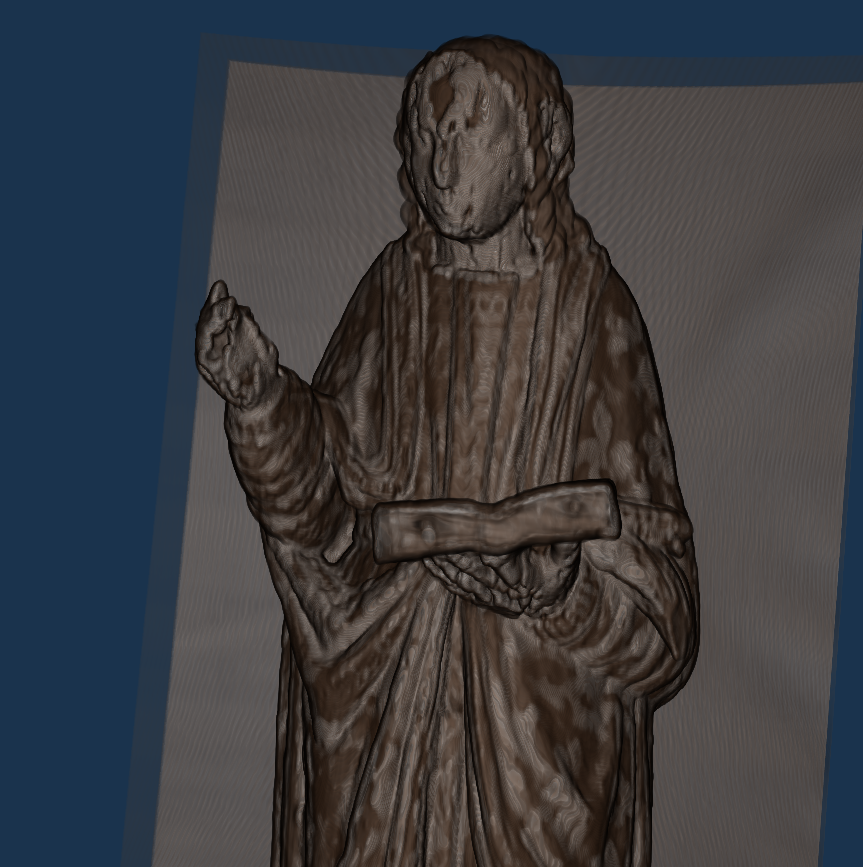
\includegraphics[width=6cm]{imagenes/resultados/filtrado/original}
	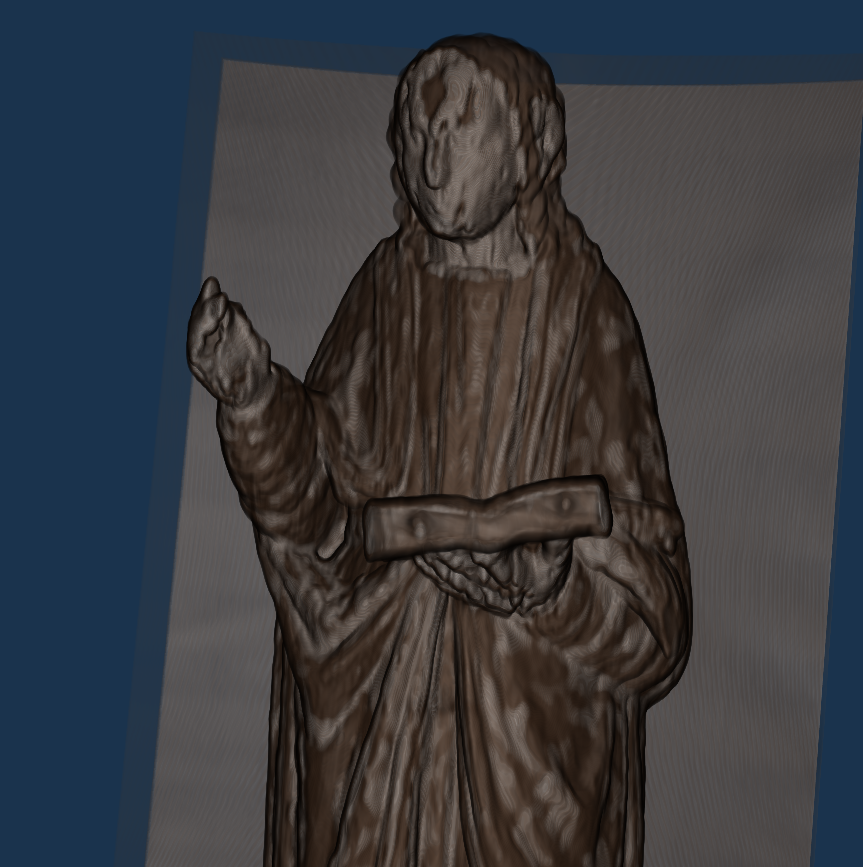
\includegraphics[width=6cm]{imagenes/resultados/filtrado/media-3}
	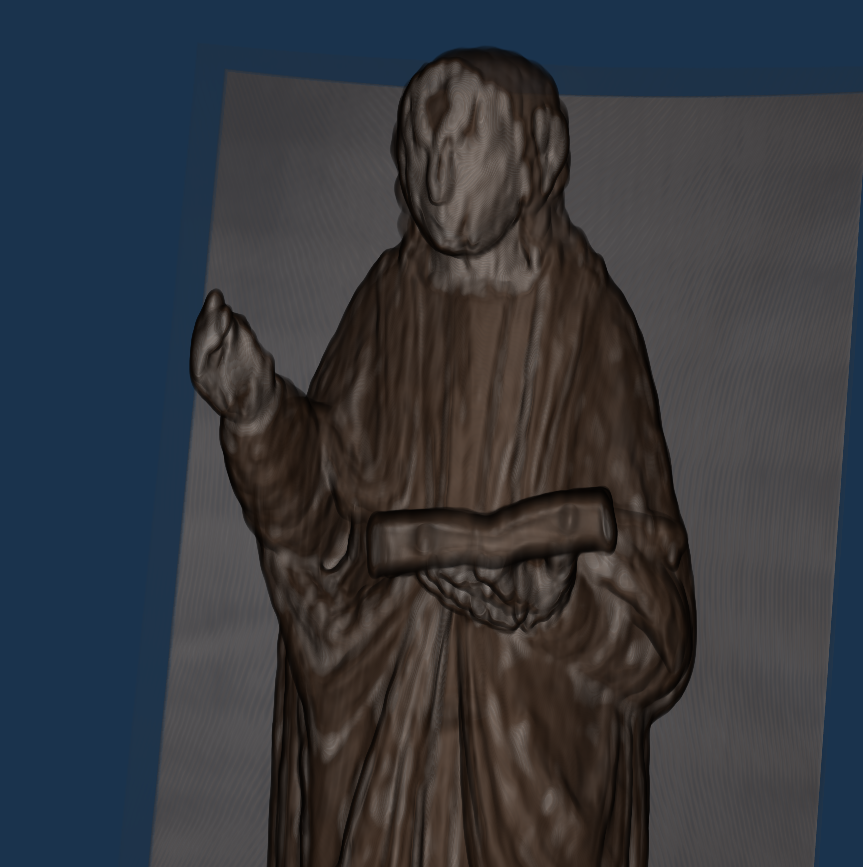
\includegraphics[width=6cm]{imagenes/resultados/filtrado/media-5}
	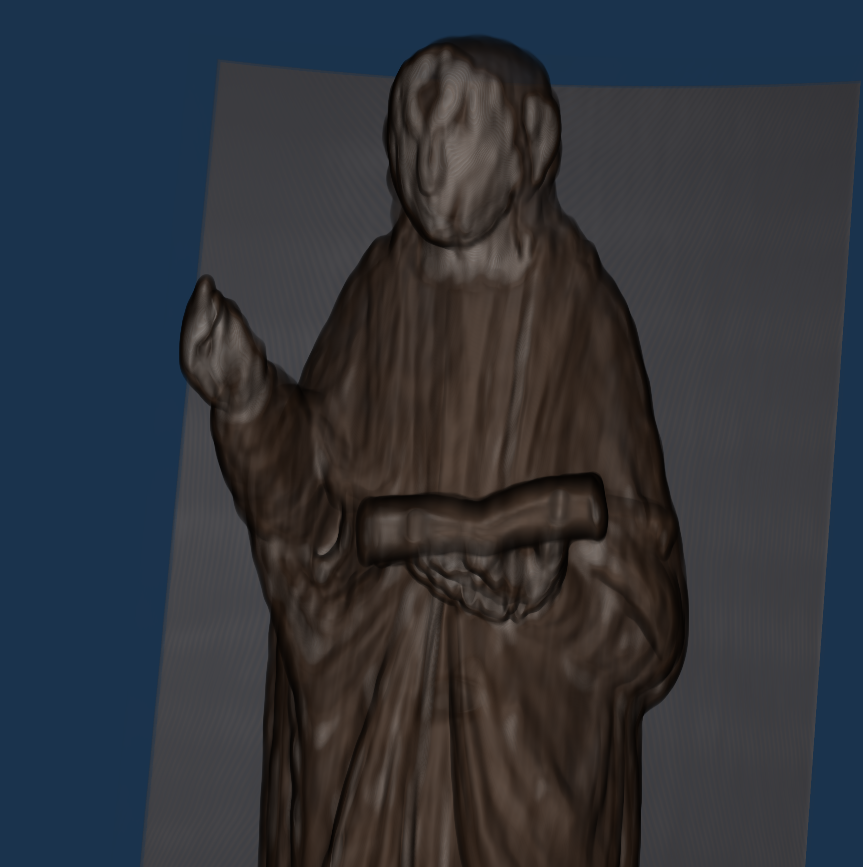
\includegraphics[width=6cm]{imagenes/resultados/filtrado/media-7}
	\caption{De izquierda a derecha y arriba a abajo: figura original y aplicando el filtro media con vecindarios de 3x3, 5x5 y 7x7}
	\label{fig:resultados/filtrado/media}
\end{figure}

Se puede ver como este filtro es bastante más agresivo que el \textit{gaussiano} y se suaviza de más. Por tanto, habría que utilizarlo para imágenes con mucho más ruido.

\subsection{Filtro mediana}

El filtro mediana se utiliza para reducir el ruido de tipo \textit{salt-and-pepper}. Nuestras imágenes no sufren de este tipo de ruido. No obstante se ha probado el filtro con vecindarios de 3x3, 5x5 y 7x7 (Figura \ref{fig:resultados/filtrado/mediana}).

\begin{figure}[H]
	\centering
	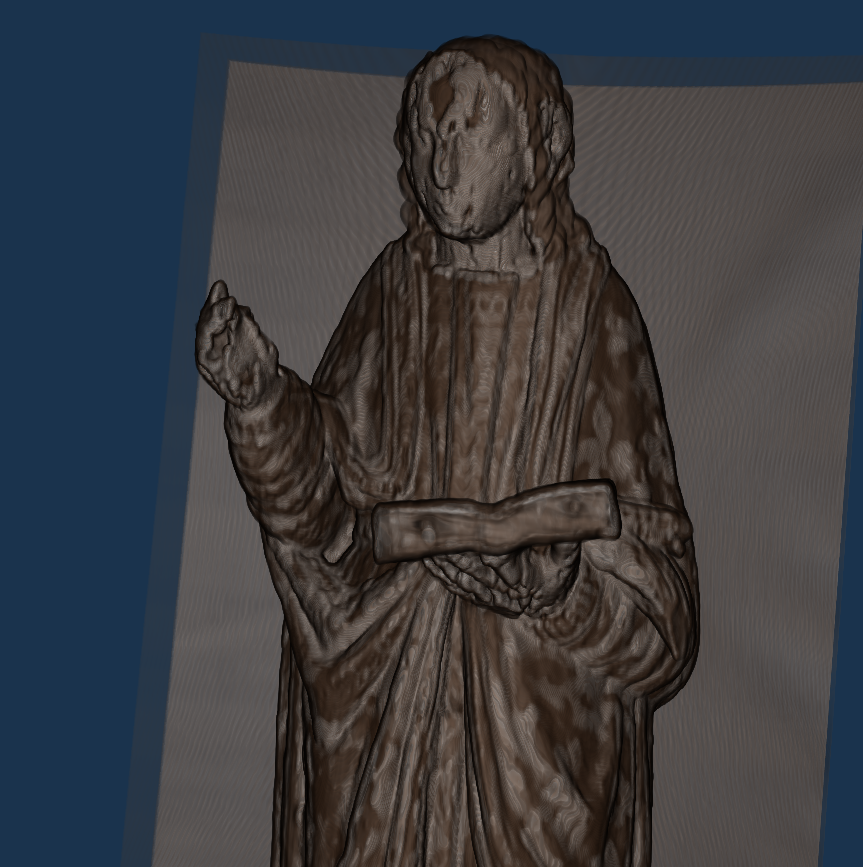
\includegraphics[width=6cm]{imagenes/resultados/filtrado/original}
	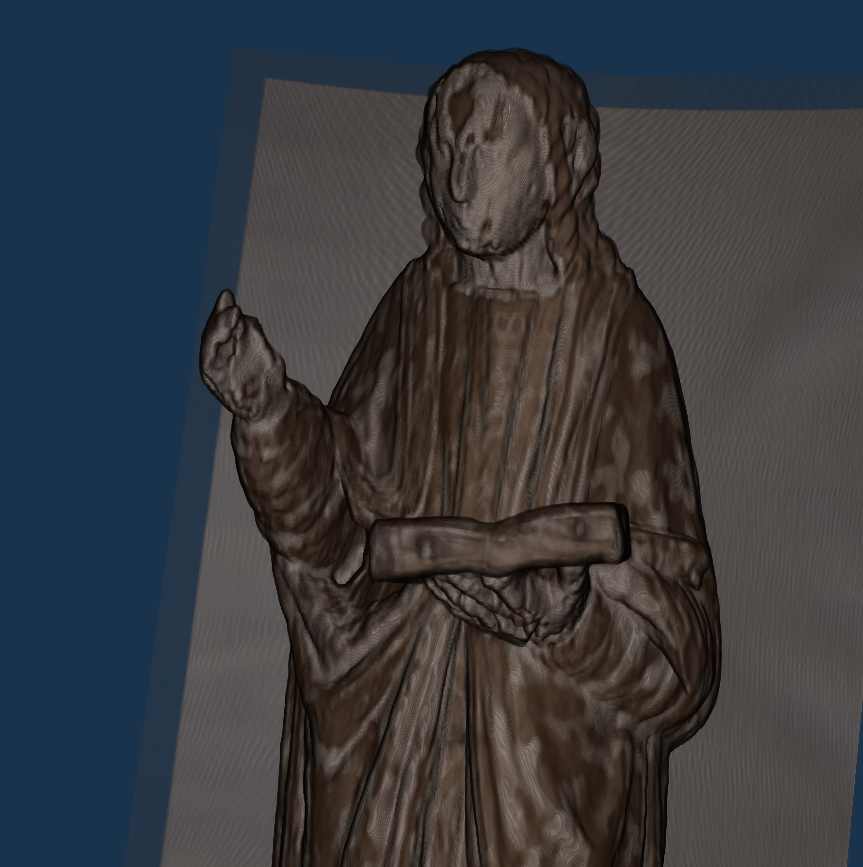
\includegraphics[width=6cm]{imagenes/resultados/filtrado/mediana-3}
	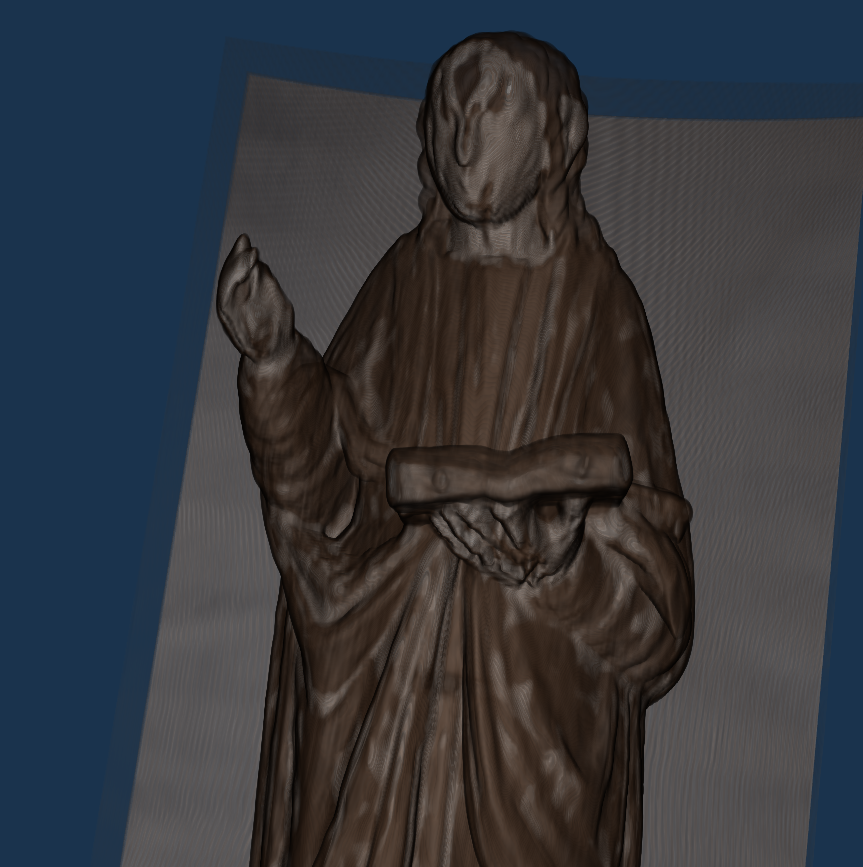
\includegraphics[width=6cm]{imagenes/resultados/filtrado/mediana-5}
	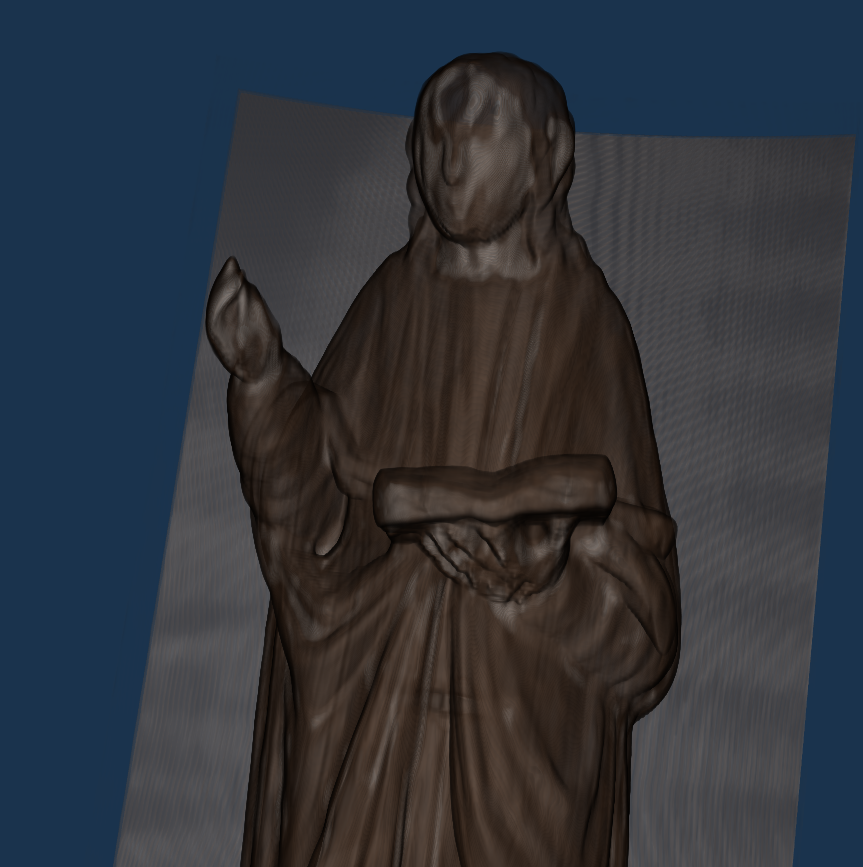
\includegraphics[width=6cm]{imagenes/resultados/filtrado/mediana-7}
	\caption{De izquierda a derecha y arriba a abajo: figura original y aplicando el filtro mediana con vecindarios de 3x3, 5x5 y 7x7}
	\label{fig:resultados/filtrado/mediana}
\end{figure}

Los resultados con este filtro son incluso más agresivos que los obtenidos con el de media. Pero es lógico al ser un filtro creado para reducir un tipo de ruido que no presentan nuestras imágenes.

\section{Segmentación}

Se ha probado el método de segmentación propuesto para separar las piezas del embón de ambas esculturas.

\subsection{Inmaculada Concepción}

En la Inmaculada Concepción hay dos piezas principales en el embón a derecha e izquierda que se puede contemplar muy bien en cualquier corte axial desde la altura del pecho hasta abajo. Por tanto se podría usar como semilla cualquiera de estos cortes pues seguramente encuentre la línea que separa ambas partes entre las líneas rectas más grandes encontradas en este corte.

Se ha utilizado uno de estos cortes y se ha encontrado fácilmente esta línea (Figura \ref{fig:resultados/segmentacion/inmaculada-concepcion/seleccion-linea}).

\begin{figure}[H]
	\centering
	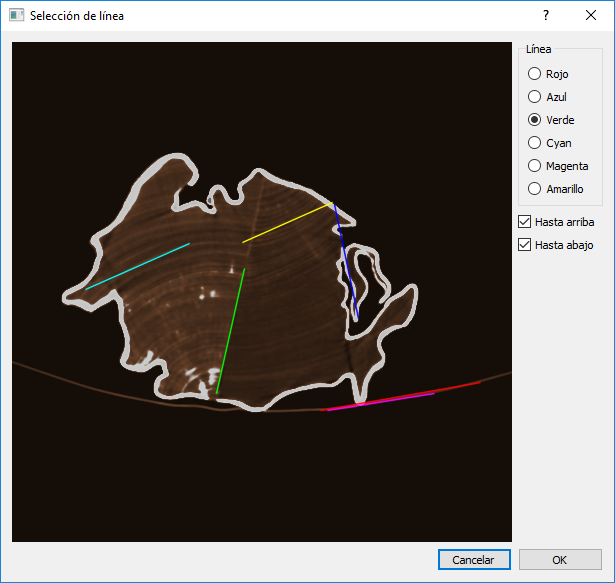
\includegraphics[width=12cm]{imagenes/resultados/segmentacion/inmaculada-concepcion/seleccion-linea}
	\caption{Líneas encontradas en un corte a la altura de la cintura donde se ve la línea (verde) que separa las dos piezas del embón}
	\label{fig:resultados/segmentacion/inmaculada-concepcion/seleccion-linea}
\end{figure}

Esta línea divide perfectamente en dos la figura obteniendo los resultados de a continuación (Figuras \ref{fig:resultados/segmentacion/inmaculada-concepcion/dcha} y \ref{fig:resultados/segmentacion/inmaculada-concepcion/dcha}).

\begin{figure}[H]
	\centering
	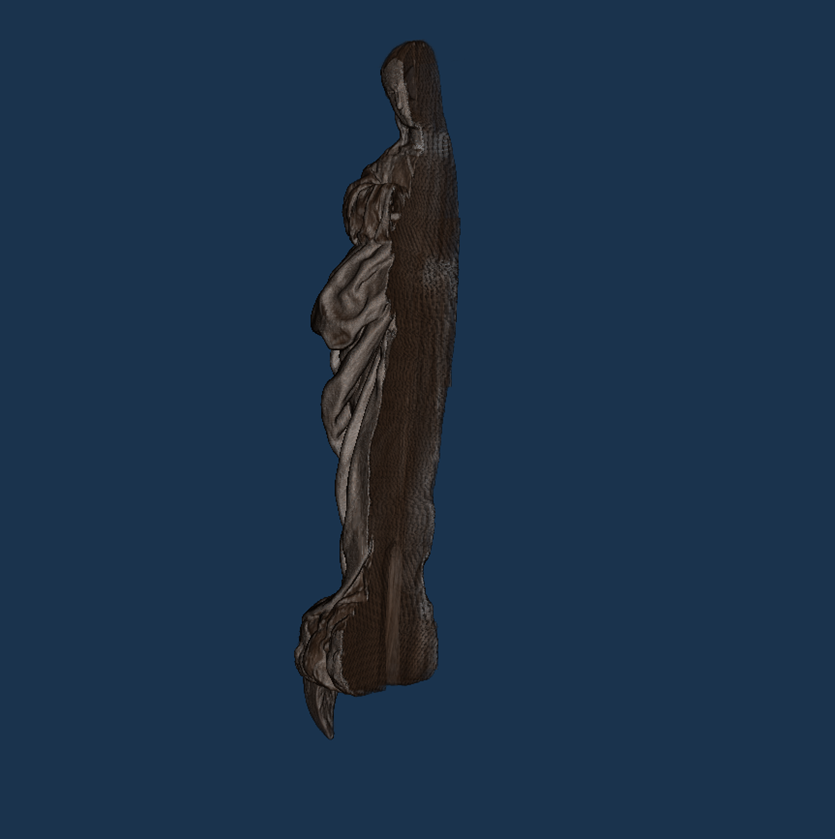
\includegraphics[width=6cm]{imagenes/resultados/segmentacion/inmaculada-concepcion/dcha-3d}
	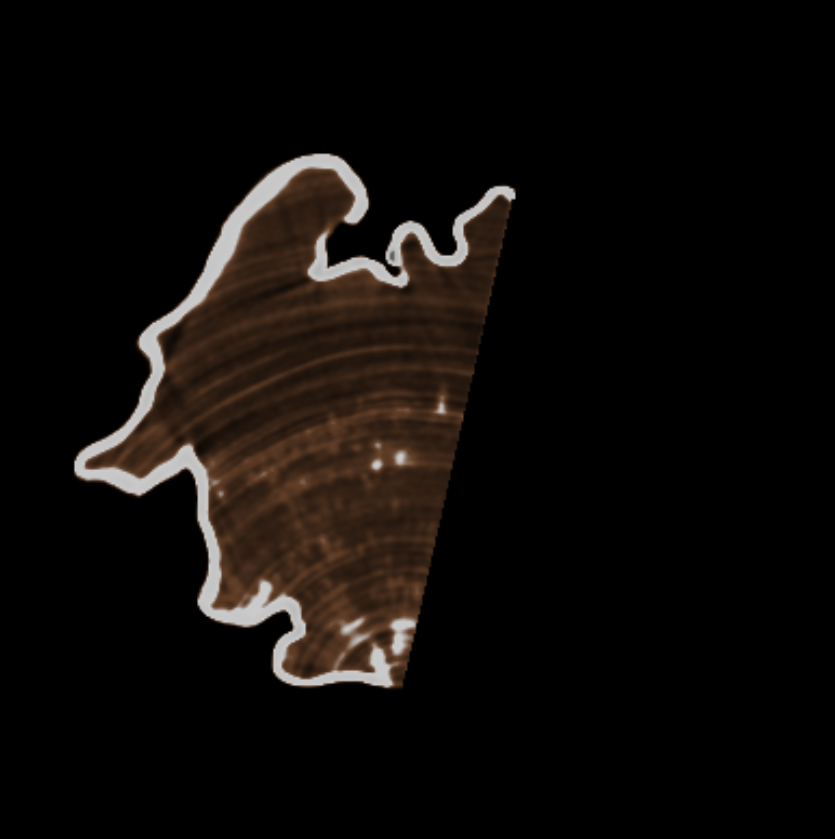
\includegraphics[width=6cm]{imagenes/resultados/segmentacion/inmaculada-concepcion/dcha-corte}
	\caption{Volumen con la pieza de la derecha y un corte donde se ve dónde ha cortado}
	\label{fig:resultados/segmentacion/inmaculada-concepcion/dcha}
\end{figure}

\begin{figure}[H]
	\centering
	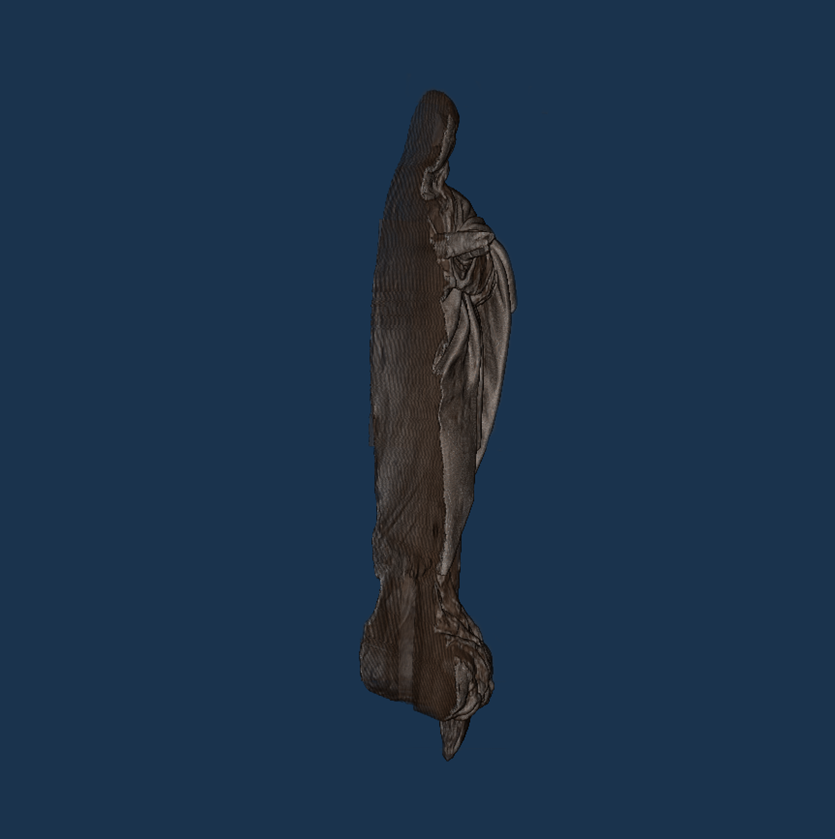
\includegraphics[width=6cm]{imagenes/resultados/segmentacion/inmaculada-concepcion/izda-3d}
	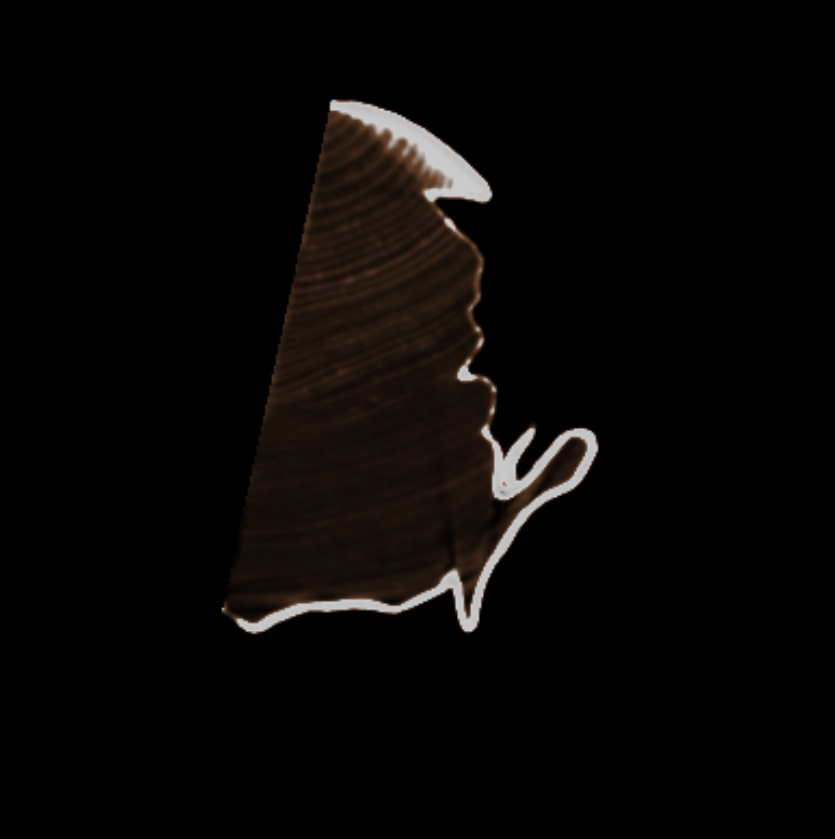
\includegraphics[width=6cm]{imagenes/resultados/segmentacion/inmaculada-concepcion/izda-corte}
	\caption{Volumen con la pieza de la izquierda y un corte donde se ve dónde ha cortado}
	\label{fig:resultados/segmentacion/inmaculada-concepcion/izda}
\end{figure}

\subsection{San Juan Evangelista}

En el San Juan Evangelista hay dos piezas principales en el embón una muy grande frontal y otra bastante más pequeña trasera. Esta pequeña no se puede ver por la zona de la cabeza y en la zona de la cintura hay un clavo que hace que no se diferencie muy bien la línea recta. Sin embargo, por la zona del pecho se puede encontrar una buena semilla donde se detecte la línea que corta ambas piezas de madera.

Se ha utilizado un corte por esta zona y se ha encontrado esta línea (Figura \ref{fig:resultados/segmentacion/inmaculada-concepcion/seleccion-linea}).

\begin{figure}[H]
	\centering
	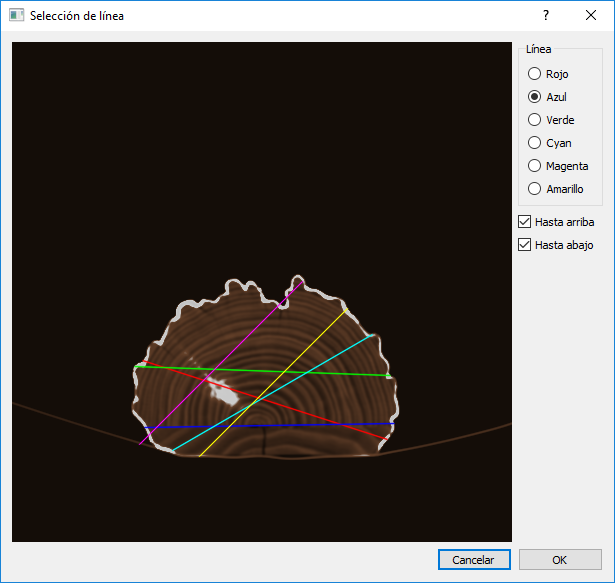
\includegraphics[width=12cm]{imagenes/resultados/segmentacion/san-juan-evangelista/seleccion-linea}
	\caption{Líneas encontradas en un corte a la altura de la cintura donde se ve la línea (azul) que separa las dos piezas del embón}
	\label{fig:resultados/segmentacion/san-juan-evangelista/seleccion-linea}
\end{figure}

Esta línea divide perfectamente en dos la figura obteniendo los resultados de a continuación (Figuras \ref{fig:resultados/segmentacion/san-juan-evangelista/frontal} y \ref{fig:resultados/segmentacion/san-juan-evangelista/trasero}).

\begin{figure}[H]
	\centering
	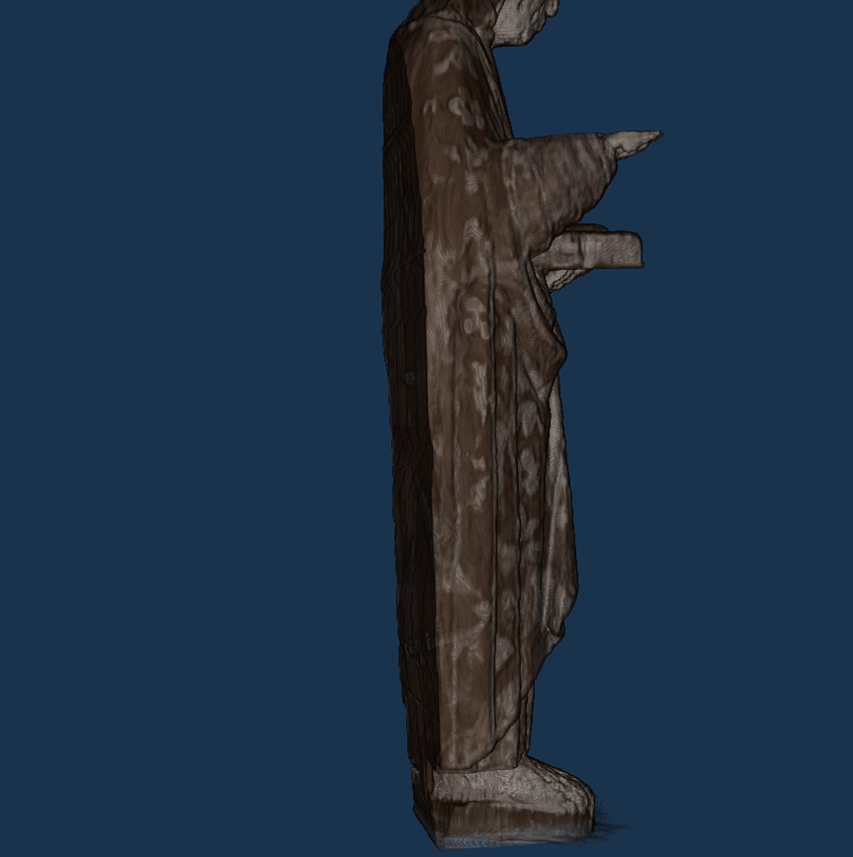
\includegraphics[width=6cm]{imagenes/resultados/segmentacion/san-juan-evangelista/frontal-3d}
	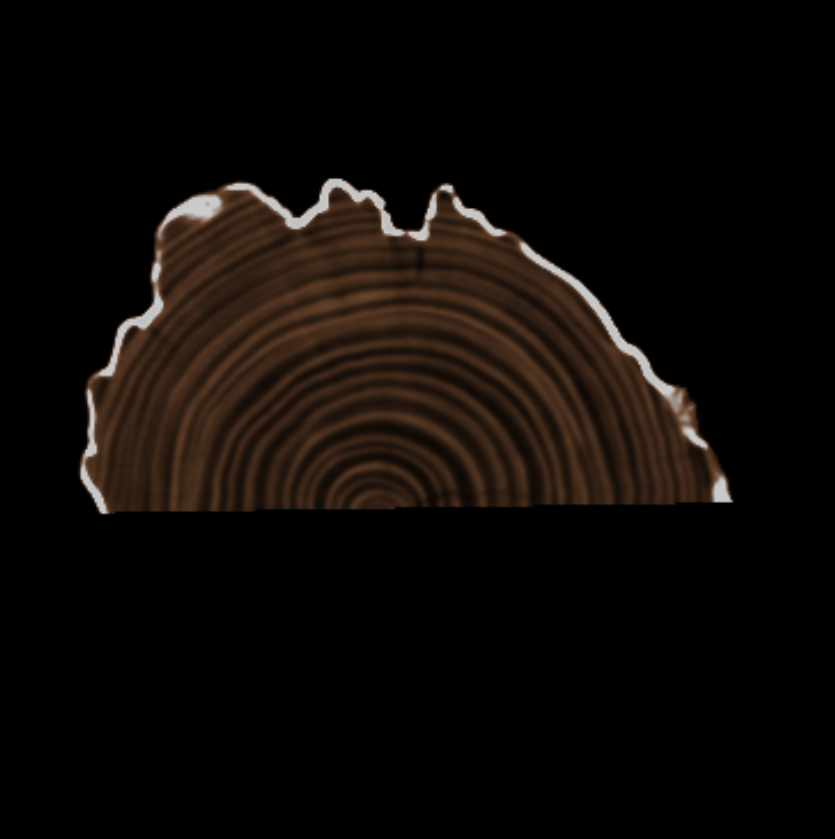
\includegraphics[width=6cm]{imagenes/resultados/segmentacion/san-juan-evangelista/frontal-corte}
	\caption{Volumen con la pieza frontal y un corte donde se ve dónde ha cortado}
	\label{fig:resultados/segmentacion/san-juan-evangelista/frontal}
\end{figure}

\begin{figure}[H]
	\centering
	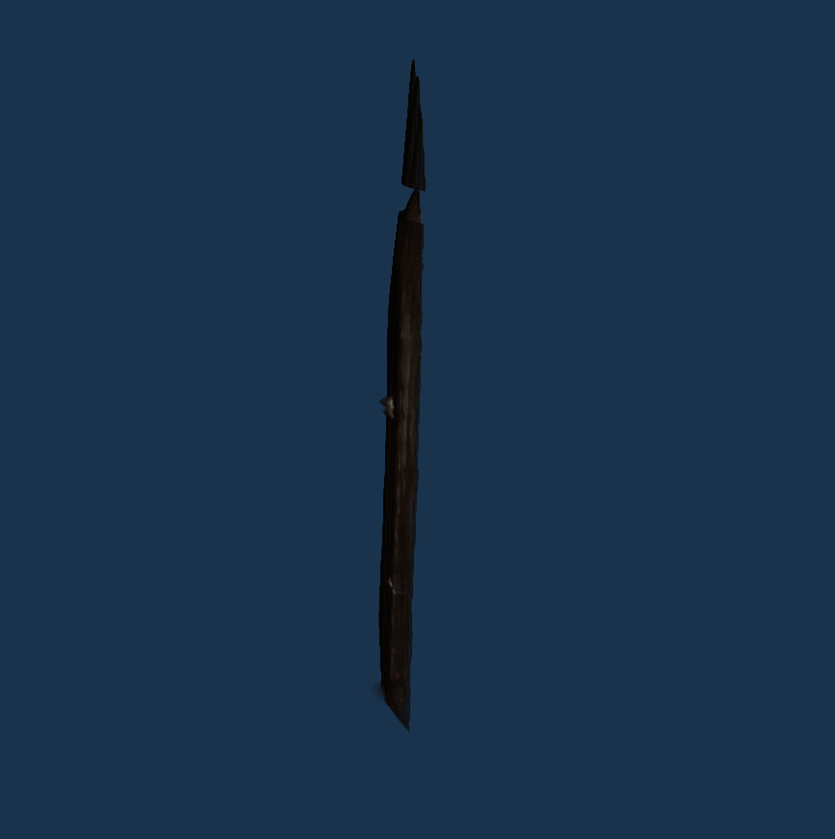
\includegraphics[width=6cm]{imagenes/resultados/segmentacion/san-juan-evangelista/trasero-3d}
	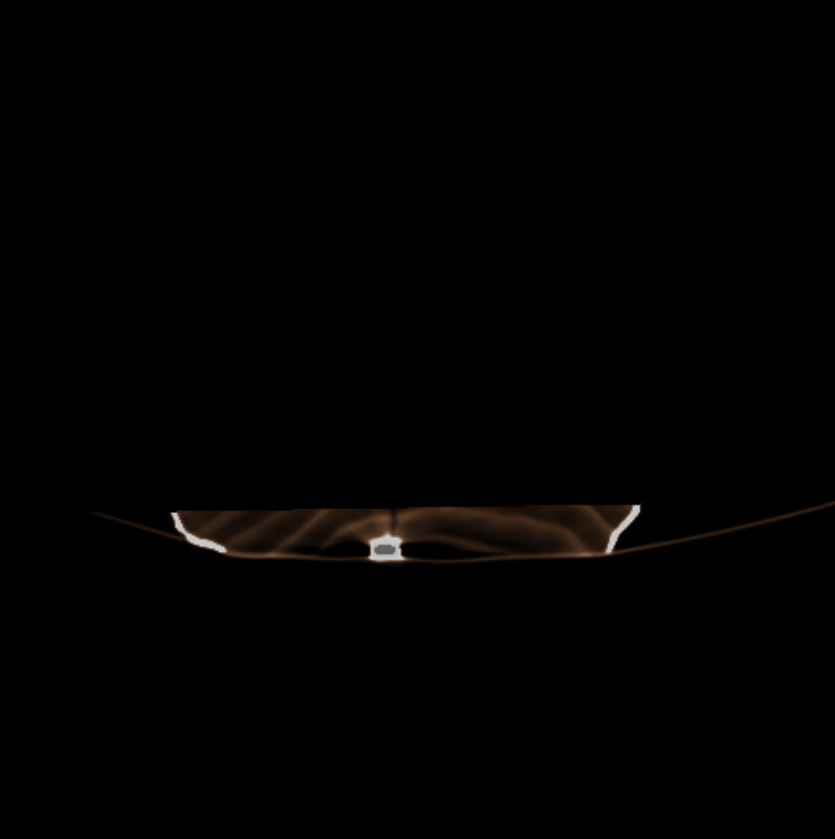
\includegraphics[width=6cm]{imagenes/resultados/segmentacion/san-juan-evangelista/trasero-corte}
	\caption{Volumen con la pieza trasera y un corte donde se ve dónde ha cortado}
	\label{fig:resultados/segmentacion/san-juan-evangelista/trasero}
\end{figure}

\section{Documentación}

En enero de 2017 tuve la oportunidad de probar el \textit{software} con las restauradoras Concha Mancebo y Amparo García de Artemisia Gestión de Patrimonio y estuvimos analizando ambas esculturas dando ellas su aportación de conocimiento técnico que yo desconozco al no haber estudiado restauración ni historia del arte.

Por ese entonces, no estaba implementado todavía el módulo de documentación y tuve que apuntar todo lo que observamos para que no se me olvidase. Esta técnica tan rudimentaria de anotación me hizo recordar la prioridad de crear un módulo específico para esto.

Al terminar este módulo, pasé todas mis anotaciones al programa para así tenerlas en este formato y en esta sección voy a utilizarlas para enseñarlas y, de paso, analizar ambas figuras pues es un ejemplo práctico muy claro del uso de 3DCurator para restauradores del arte.

\subsection{Inmaculada Concepción}

En primer lugar se hizo un estudio de las dimensiones de esta pieza que tiene una altura de 59cm y un hueco donde colocar el soporte de 12,5cm (Figura \ref{fig:resultados/documentacion/inmaculada-concepcion/sagital}).

\begin{figure}[H]
	\centering
	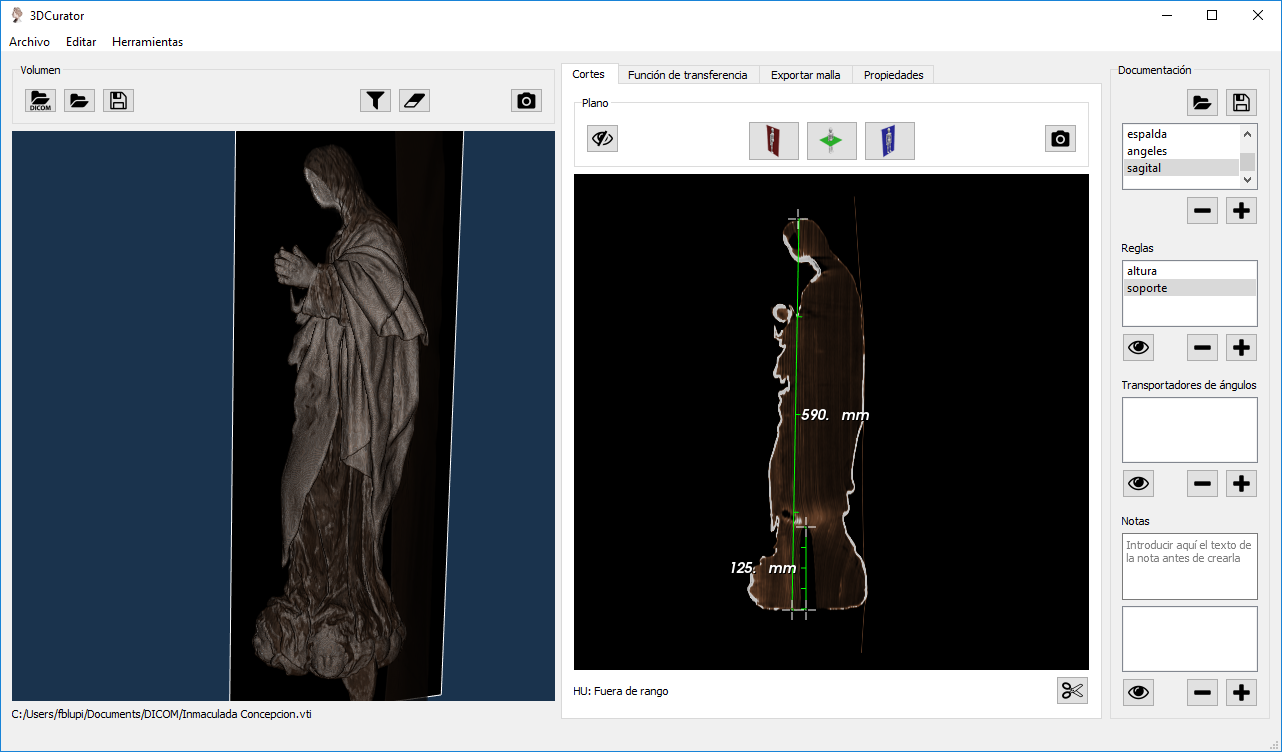
\includegraphics[width=12.5cm]{imagenes/resultados/documentacion/inmaculada-concepcion/sagital}
	\caption{Corte sagital para ver el tamaño de la escultura}
	\label{fig:resultados/documentacion/inmaculada-concepcion/sagital}
\end{figure}

A continuación se realizó una observación con el plano axial de arriba a abajo para ir analizando uno a uno los elementos que nos fuésemos encontrando.

En primer lugar nos encontramos con la cabeza donde se ven tres piezas de madera: La pieza del rostrillo y otras dos y el hueco donde están los ojos de cristal.

En el rostro se observa también lo que puede parecer un repolicromado sobre una capa de policromía con blanco de plomo pues se observa un elemento metálico(Figura \ref{fig:resultados/documentacion/inmaculada-concepcion/cabeza}).

\begin{figure}[H]
	\centering
	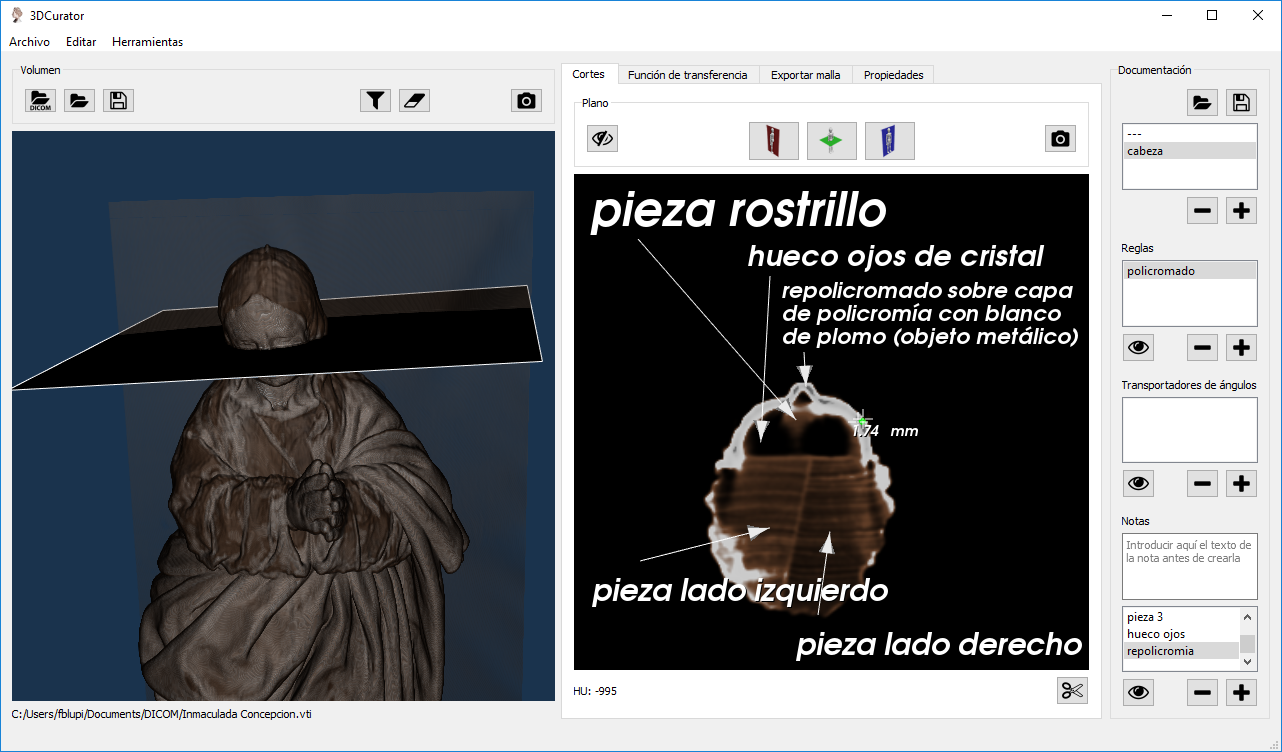
\includegraphics[width=12.5cm]{imagenes/resultados/documentacion/inmaculada-concepcion/cabeza}
	\caption{Corte axial a la altura de la cabeza donde analizamos sus elementos}
	\label{fig:resultados/documentacion/inmaculada-concepcion/cabeza}
\end{figure}

En el cuello desaparece la pieza del rostrillo y se ven dos piezas que se mantienen hasta el final de la pieza pues son las que, claramente, forman el embón. También se puede ver bastante ruido producido por los elementos metálicos como el blanco de plomo (Figura \ref{fig:resultados/documentacion/inmaculada-concepcion/cuello}).

\begin{figure}[H]
	\centering
	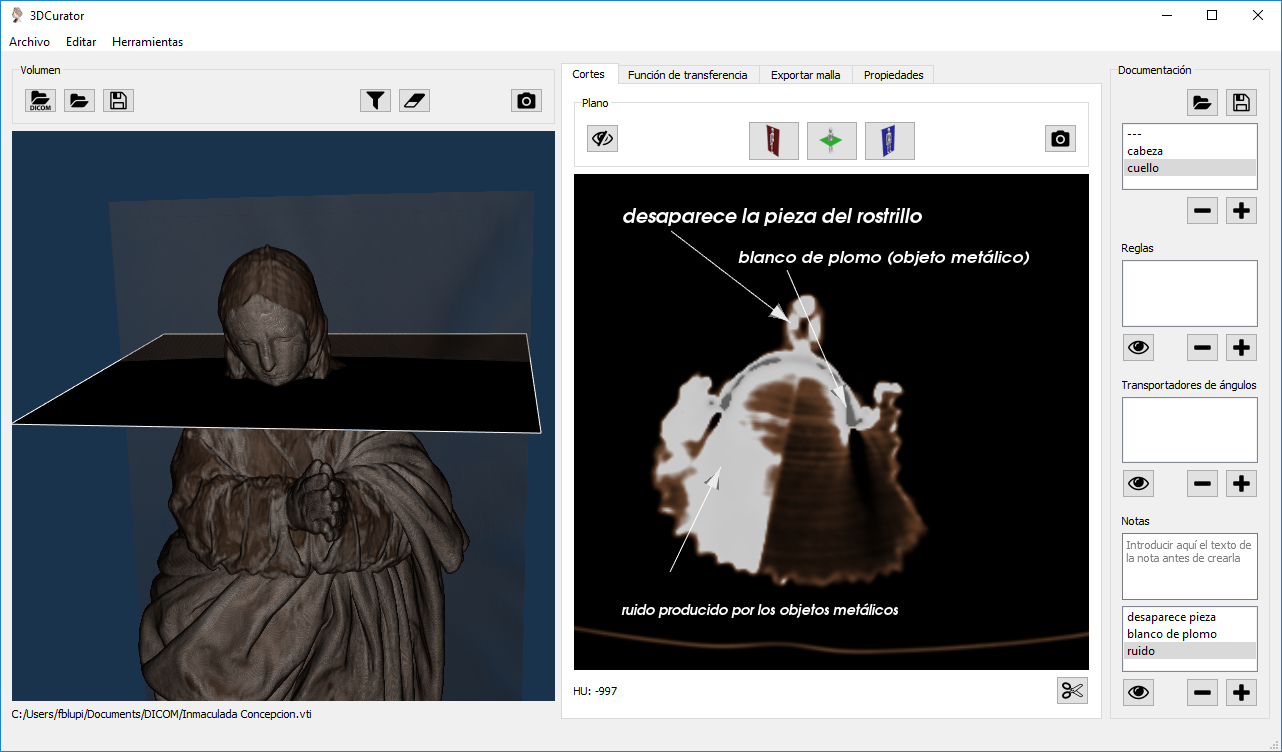
\includegraphics[width=12.5cm]{imagenes/resultados/documentacion/inmaculada-concepcion/cuello}
	\caption{Corte axial a la altura del cuello donde analizamos sus elementos}
	\label{fig:resultados/documentacion/inmaculada-concepcion/cuello}
\end{figure}

Más abajo, llegamos a las manos donde se puede ver mucho estuco, lo cual extraña bastante a las restauradoras ya que, al haber tenido una experiencia previa restaurando la escultura, se ha podido ver que la capa de estuco que tenían era muy fina por lo que el estuco que se observa en la imagen tiene que ser ruido producido, seguramente, por el blanco de plomo de la policromía de la carnación o porque se le añadió blanco de plomo como carga al estuco.

Se puede observar también el empiezado de las manos que son dos piezas independientes. Van encajadas y encoladas sin usar ninguna punta (Figura \ref{fig:resultados/documentacion/inmaculada-concepcion/manos}).

\begin{figure}[H]
	\centering
	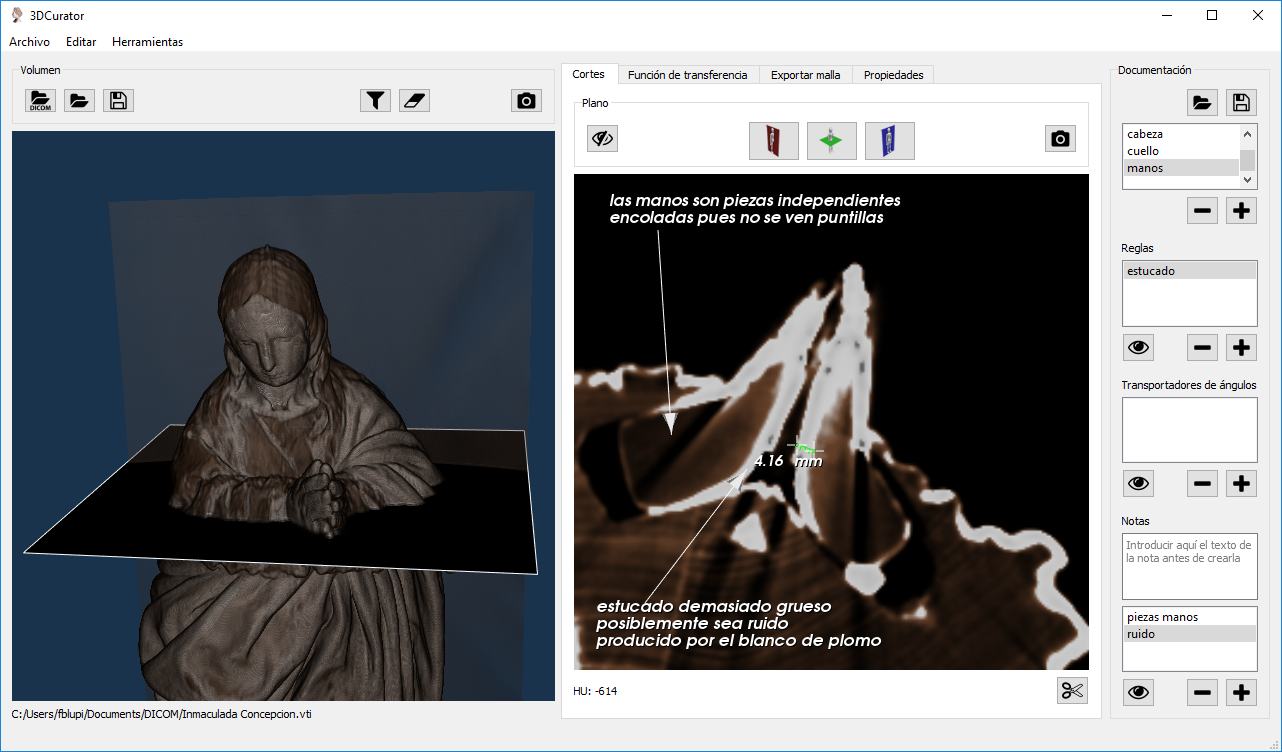
\includegraphics[width=12.5cm]{imagenes/resultados/documentacion/inmaculada-concepcion/manos}
	\caption{Corte axial a la altura de las manos donde analizamos sus elementos}
	\label{fig:resultados/documentacion/inmaculada-concepcion/manos}
\end{figure}

En la parte del manto donde hay bastantes pliegues se ve una capa de estuco bastante más gruesa que en el resto de la pieza. En la parte de atrás se encuentra todavía el pelo que apenas tiene estuco (Figura \ref{fig:resultados/documentacion/inmaculada-concepcion/pecho}).

\begin{figure}[H]
	\centering
	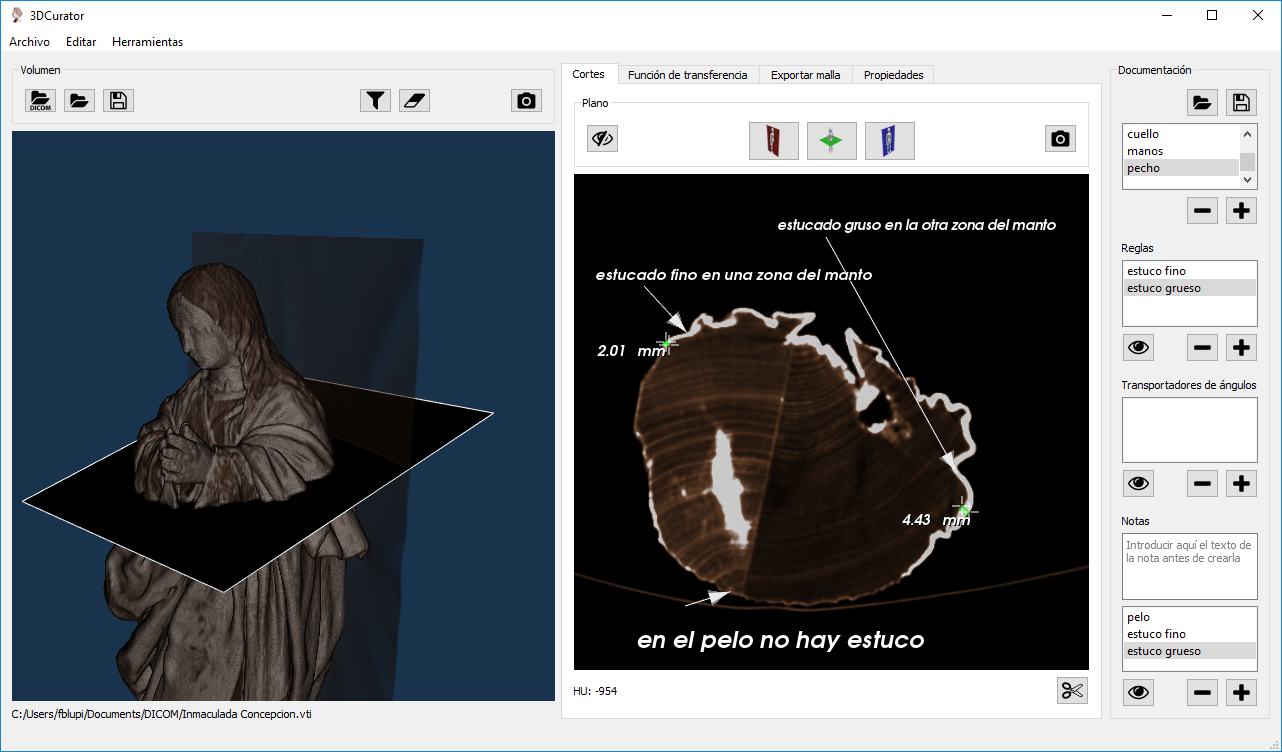
\includegraphics[width=12.5cm]{imagenes/resultados/documentacion/inmaculada-concepcion/pecho}
	\caption{Corte a la altura del pecho donde analizamos sus elementos}
	\label{fig:resultados/documentacion/inmaculada-concepcion/pecho}
\end{figure}

Justo antes de alcanzar el agujero donde se coloca el soporte para apoyar la escultura se observan zonas del embón que están algo más abiertas. 

La causa exacta que ha provocado la grieta no se puede saber con certeza, pero puede haber sido producida:

\begin{itemize}
	\item o por la presión producida cuando se realizó el agujero donde se coloca el soporte de la figura (de un diámetro de aproximadamente 21,6mm) que haya hecho que salte madera.
	\item o porque tuviera un poco de deformación y al secarse el adhesivo se generase un hueco ahí.
\end{itemize}

Pero esto no genera ningún riesgo porque como son dos piezas bien adheridas por el resto de la figura y no se ha producido ningún movimiento.

\begin{figure}[H]
	\centering
	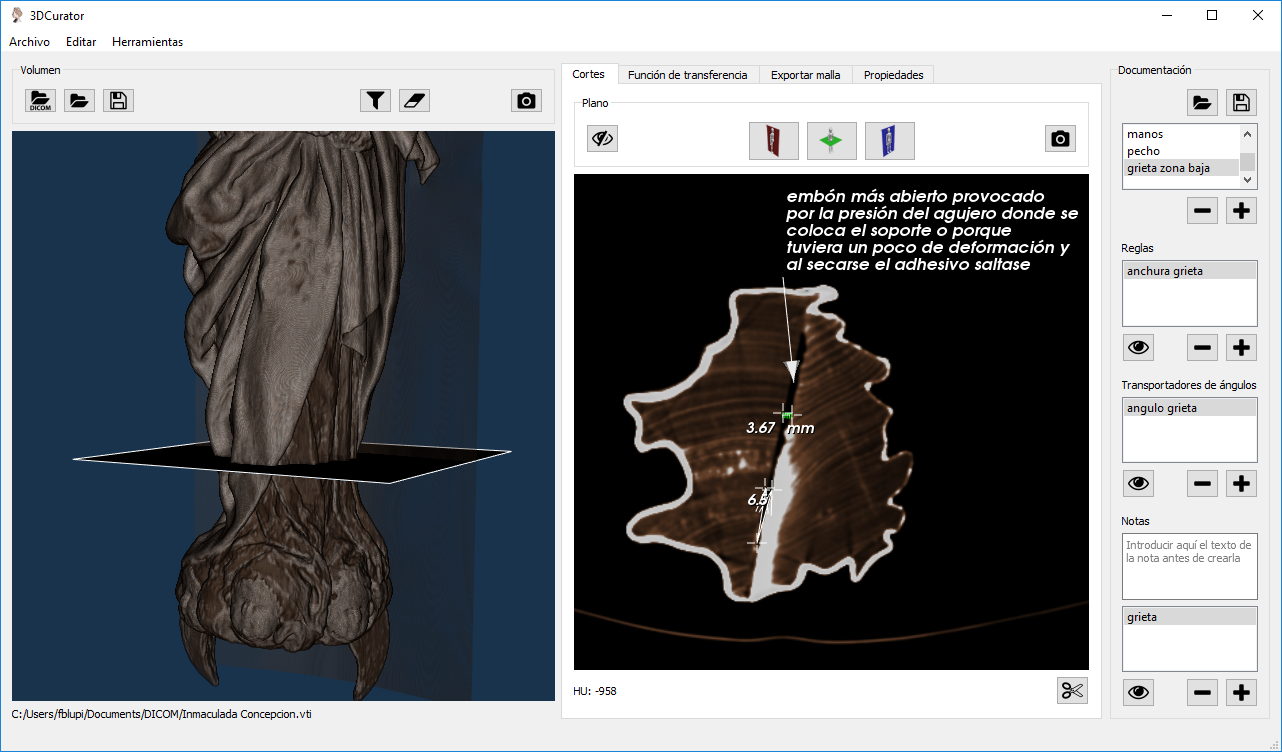
\includegraphics[width=12.5cm]{imagenes/resultados/documentacion/inmaculada-concepcion/grieta-zona-baja}
	\caption{Corte axial justo por encima del final del agujero para el soporte donde analizamos la grieta que se ve}
	\label{fig:resultados/documentacion/inmaculada-concepcion/grieta-zona-baja}
\end{figure}

Un poco más arriba, desde fuera sí se observaba una grieta en la espalda (que también se puede ver tanto en cortes generados con el plano como en la vista en 3D), aunque es bastante más fina que la que se ha observado previamente. Cerca tiene un nudo la madera, por lo que puede que haya sido producido por éste.

\begin{figure}[H]
	\centering
	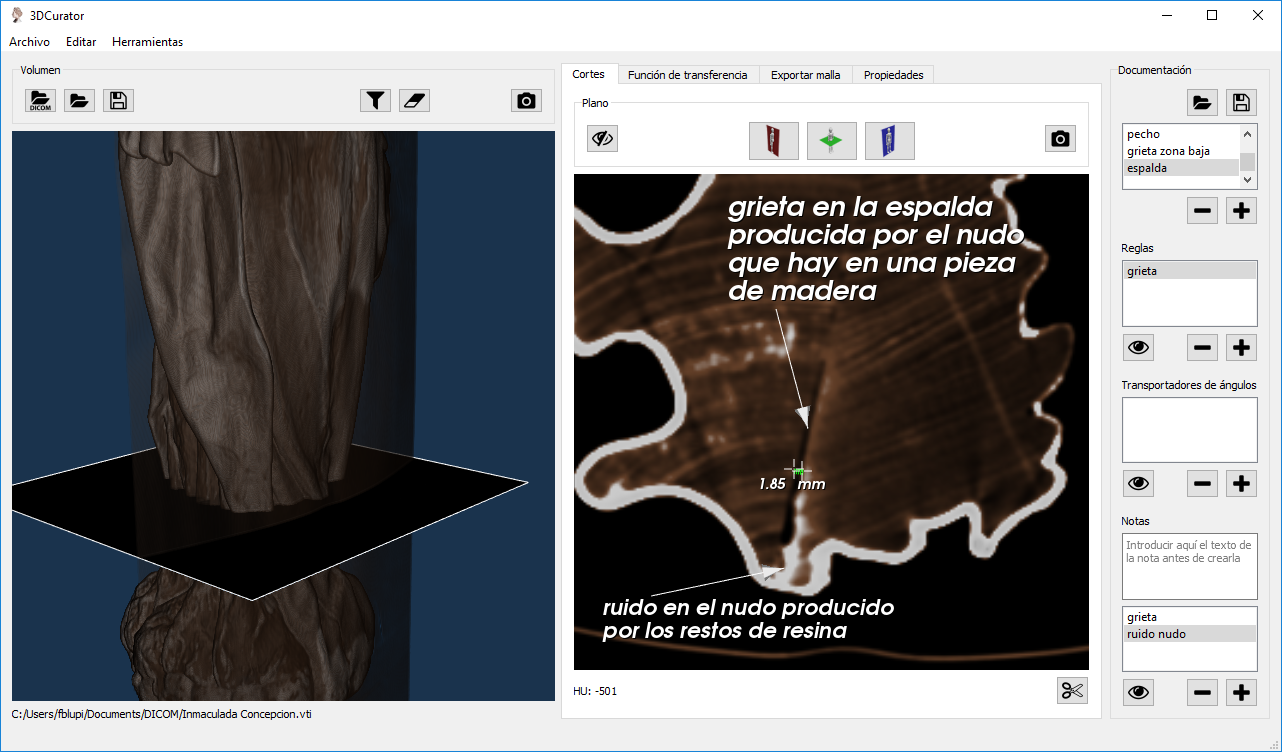
\includegraphics[width=12.5cm]{imagenes/resultados/documentacion/inmaculada-concepcion/espalda}
	\caption{Corte axial en la espalda donde se puede observar otra pequeña grieta}
	\label{fig:resultados/documentacion/inmaculada-concepcion/espalda}
\end{figure}

Más abajo, llegamos ya a la zona de las nubes y los ángeles donde podemos encontrar muchos elementos interesantes.

Se vuelve a ver en las carnaciones de las cabezas de los ángeles zonas con metal, lo que refuerza la teoría de que éstas están hechas con blanco de plomo.

La cara del ángel frontal está en una pieza distinta a las dos que vienen formando la escultura completa. Puede que esta pieza de madera formase parte del embón original hasta arriba aunque solo haya sido usado en esta zona inferior (o incluso en la cara) y al irse tallando solo se encuentre aquí o que se haya adherido posteriormente.

En cambio, los cuernos de luna si se nota que han sido añadidos posteriormente empiezados y sin usar puntillas.

Inesperadamente no se aprecia la capa de pan de oro en los cuernos y es que o es tan fino que el escáner no lo detecta con tanta precisión o al ser un material tan denso no esté preparado para capturar este material.

Se puede ver también un nudo en la madera lo cual no se puede ver con ninguna otra técnica. En este nudo se ve también brillo posiblemente producido por restos de resina (Figura \ref{fig:resultados/documentacion/inmaculada-concepcion/angeles}). 

\begin{figure}[H]
	\centering
	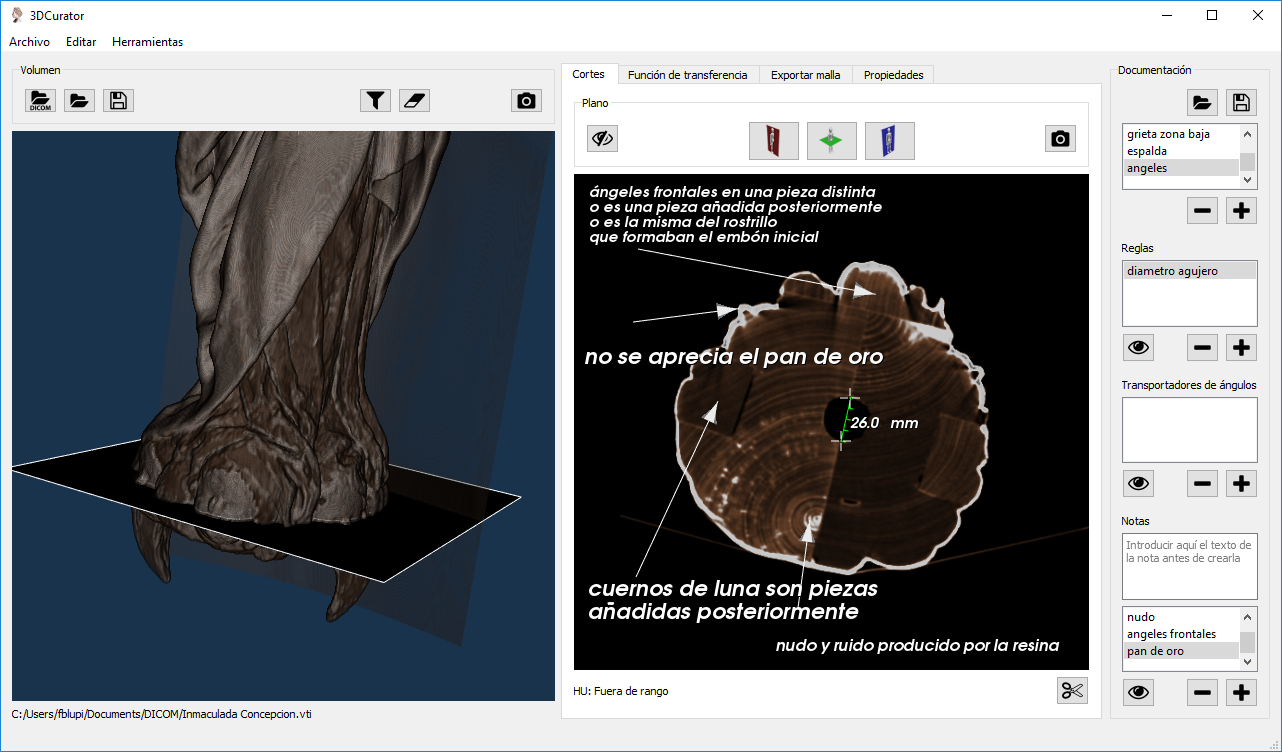
\includegraphics[width=12.5cm]{imagenes/resultados/documentacion/inmaculada-concepcion/angeles}
	\caption{Corte axial en la zona de los ángeles donde analizamos todos sus elementos}
	\label{fig:resultados/documentacion/inmaculada-concepcion/angeles}
\end{figure}

\subsection{San Juan Evangelista}

Al igual que con la primera figura, se ha hecho en primer lugar un estudio de sus dimensiones y mide poco más de medio metro (Figura \ref{fig:resultados/documentacion/san-juan-evangelista/sagital}). 

\begin{figure}[H]
	\centering
	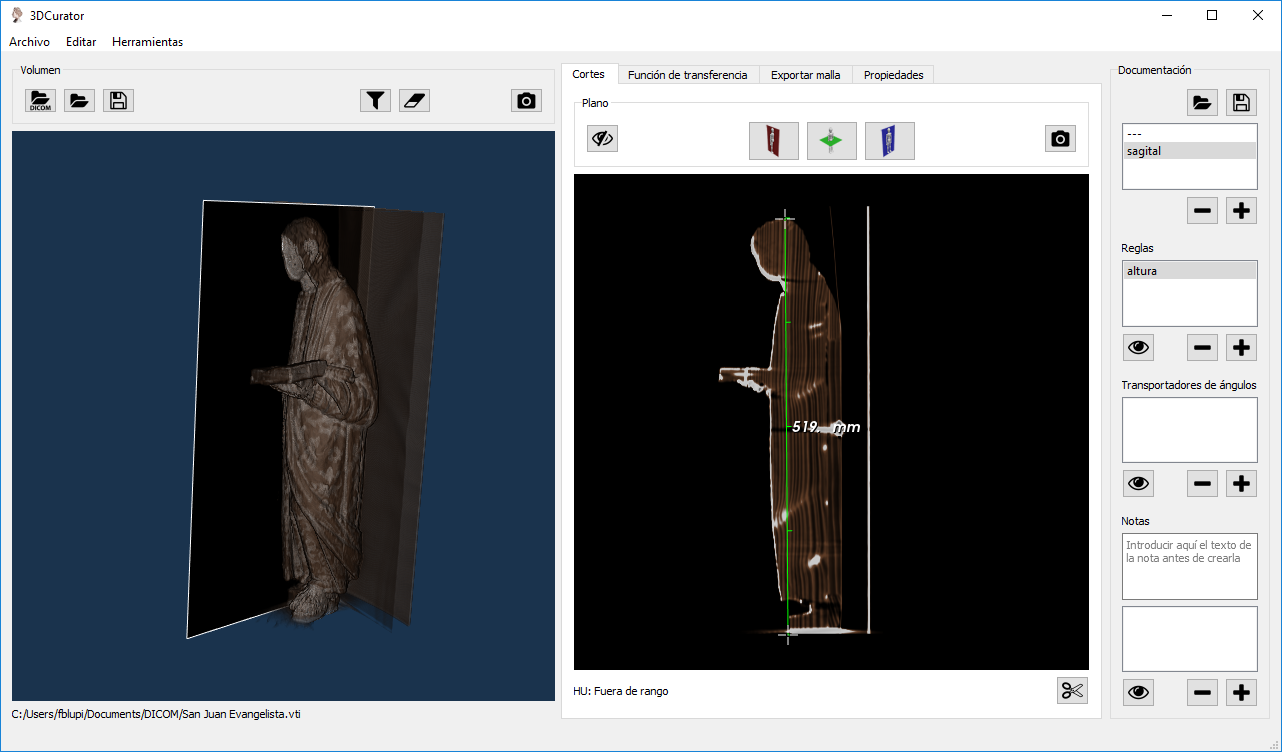
\includegraphics[width=12.5cm]{imagenes/resultados/documentacion/san-juan-evangelista/sagital}
	\caption{Corte sagital para estudiar la altura de la figura}
	\label{fig:resultados/documentacion/san-juan-evangelista/sagital}
\end{figure}

Esta figura tiene mucho pan de oro: en el manto, el vestido, el libro... También se observa bastante más ruido en toda la figura (en la reconstrucción en 3D es tremendamente apreciable), posiblemente producido por esto.

En las carnaciones de esta figura se vuelve a apreciar el mismo ruido que en el de las de la otra escultura. En cambio, ni en el pelo ni en toda la zona trasera se aprecia estuco (Figura \ref{fig:resultados/documentacion/san-juan-evangelista/cabeza}). 

\begin{figure}[H]
	\centering
	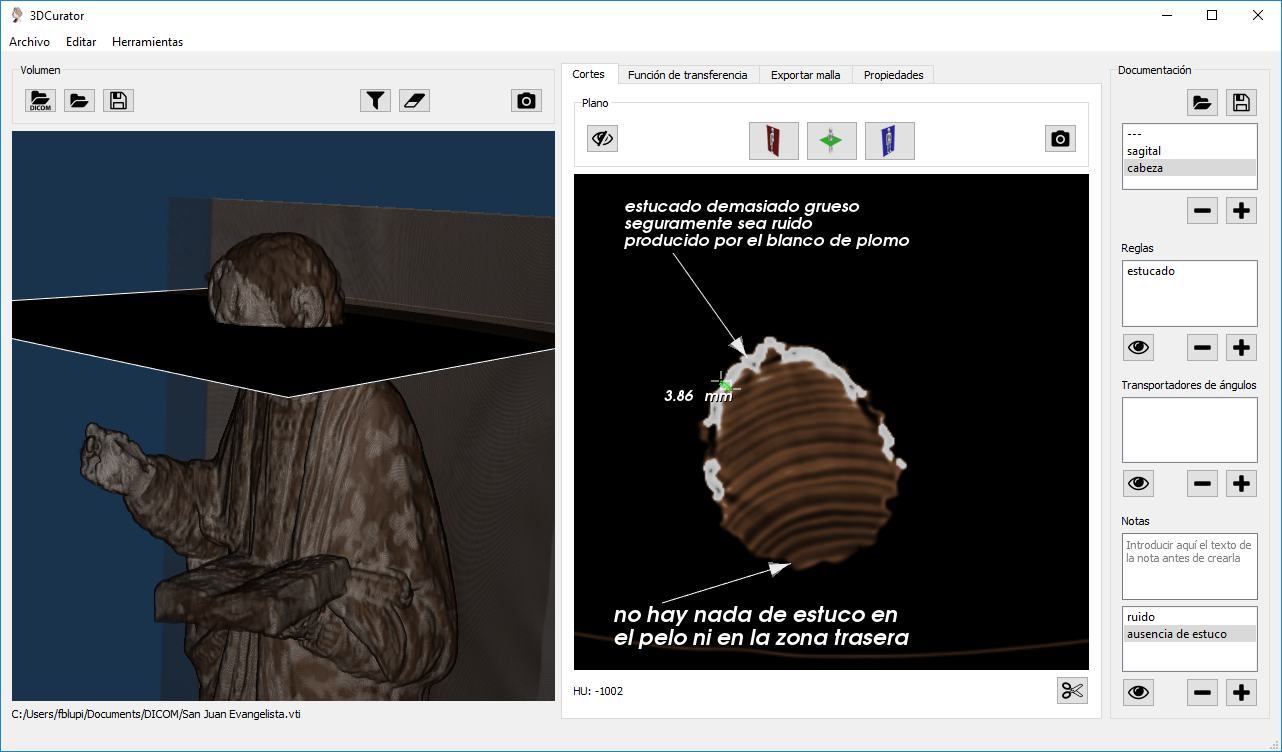
\includegraphics[width=12.5cm]{imagenes/resultados/documentacion/san-juan-evangelista/cabeza}
	\caption{Corte axial en la zona de la cabeza para estudiar su composición}
	\label{fig:resultados/documentacion/san-juan-evangelista/cabeza}
\end{figure}

Una vez pasada la cabeza se puede ver la composición del embón. Son dos piezas de madera distintas, aunque la segunda (la que se encuentra en la parte trasera) es bastante más fina.

Si se observa con detalle el libro, se puede ver que hay otra pieza más de madera ahí, unida con pequeñas puntillas, posiblemente adheridas en una intervención pues podría estar originalmente encolado (Figura \ref{fig:resultados/documentacion/san-juan-evangelista/libro}). 

\begin{figure}[H]
	\centering
	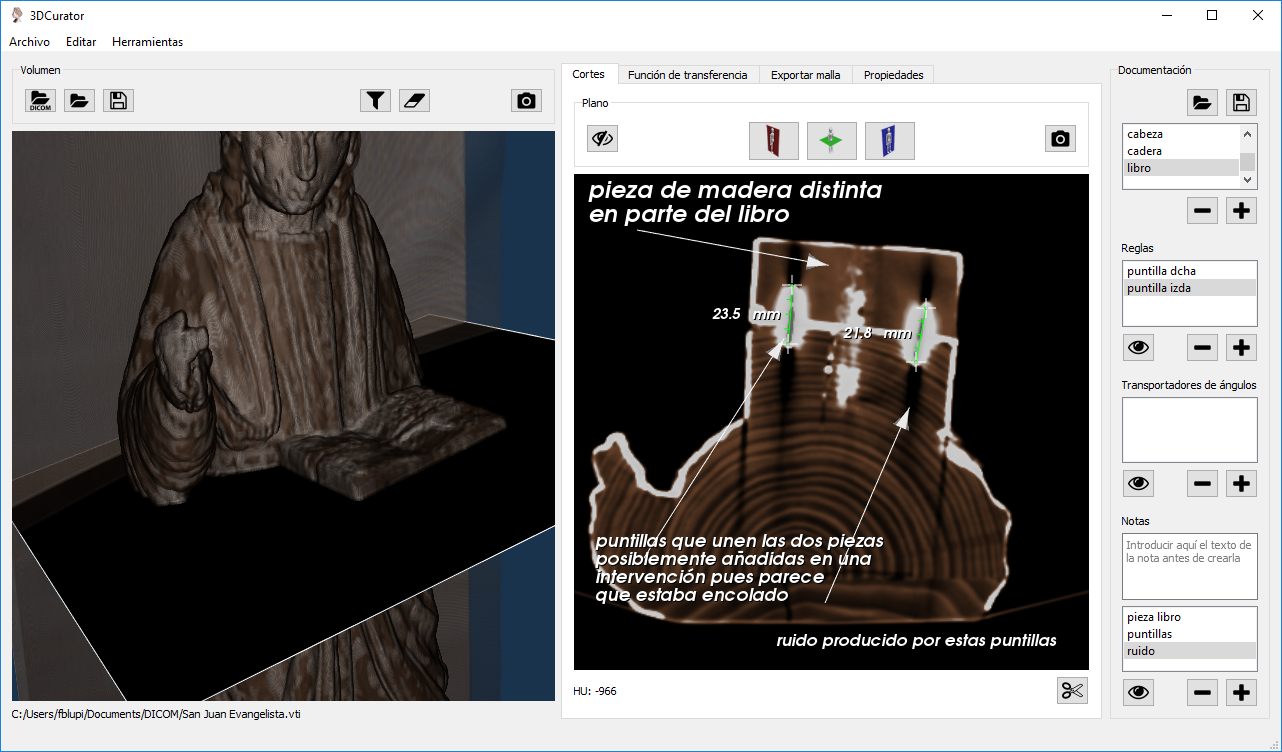
\includegraphics[width=12.5cm]{imagenes/resultados/documentacion/san-juan-evangelista/libro}
	\caption{Corte a la altura del libro y con una orientación arbitraria para poder apreciar cómo está unido con la pieza de madera principal}
	\label{fig:resultados/documentacion/san-juan-evangelista/libro}
\end{figure}

En la reconstrucción en 3D se puede ver que faltan dedos en la mano derecha. En la intervención no se restauraron, solo se limpiaron los cortes que se ven bastante suavizados.

Antes de llegar al clavo principal que une las dos piezas del embón se puede ver una grieta, posiblemente producida por éste (Figura \ref{fig:resultados/documentacion/san-juan-evangelista/cadera}). 

\begin{figure}[H]
	\centering
	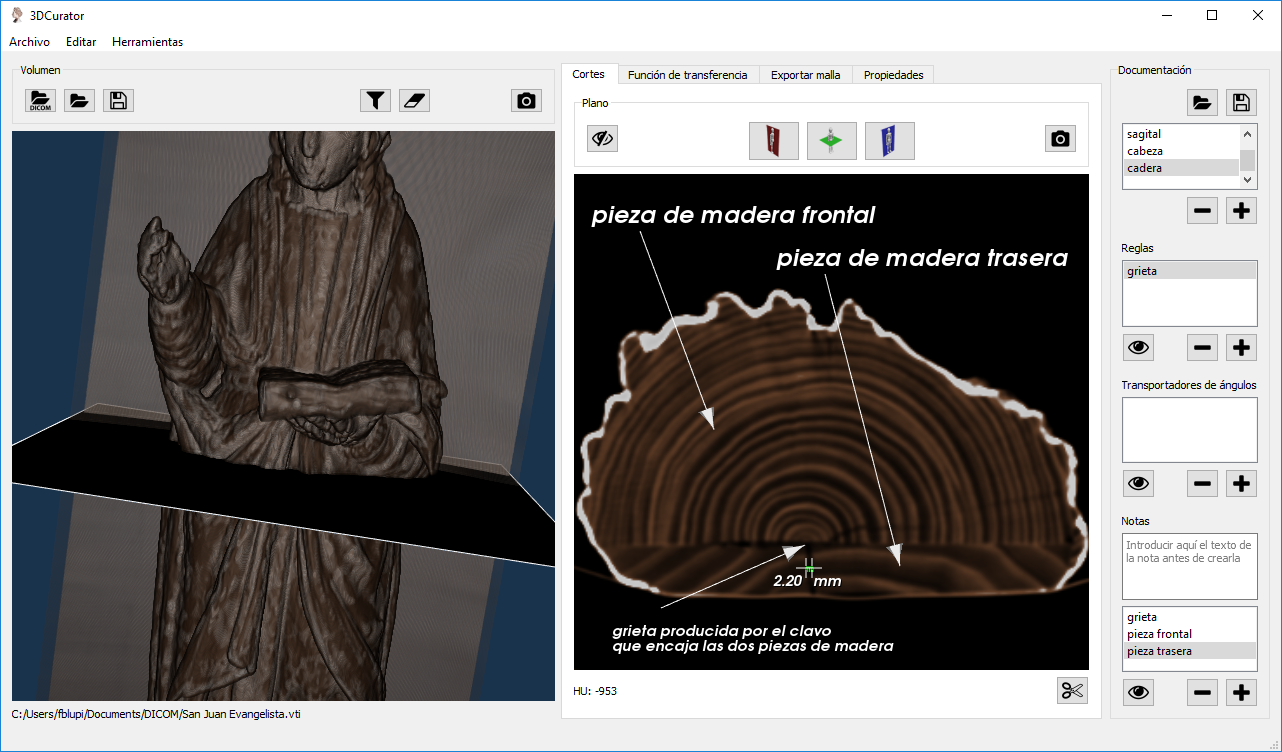
\includegraphics[width=12.5cm]{imagenes/resultados/documentacion/san-juan-evangelista/cadera}
	\caption{Corte axial a la altura de la cadera antes de llegar al clavo donde se puede ver una grieta producida por éste}
	\label{fig:resultados/documentacion/san-juan-evangelista/cadera}
\end{figure}

El clavo grande que une las dos piezas de madera que forman el embón se ve muy bien, aunque produce mucho ruido se puede ver que está entero (Figura \ref{fig:resultados/documentacion/san-juan-evangelista/clavo-central}). 

\begin{figure}[H]
	\centering
	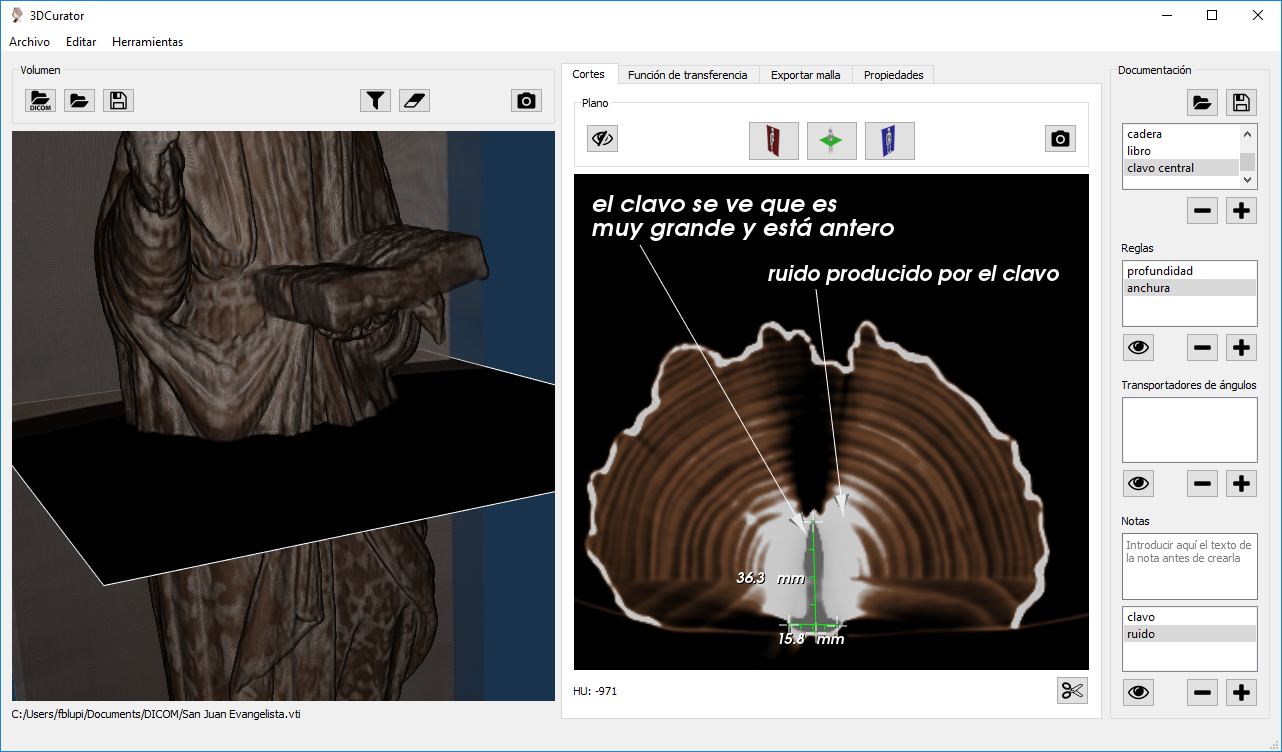
\includegraphics[width=12.5cm]{imagenes/resultados/documentacion/san-juan-evangelista/clavo-central}
	\caption{Corte axial a la altura del clavo que une las dos piezas del embón}
	\label{fig:resultados/documentacion/san-juan-evangelista/clavo-central}
\end{figure}

Más abajo hay otros dos clavos más, a la altura de las rodillas por la parte trasera. A uno de ellos le falta la cabeza. Puede que lo hayan intentado sacar y no lo hayan logrado (Figura \ref{fig:resultados/documentacion/san-juan-evangelista/clavos-rodillas}). 

\begin{figure}[H]
	\centering
	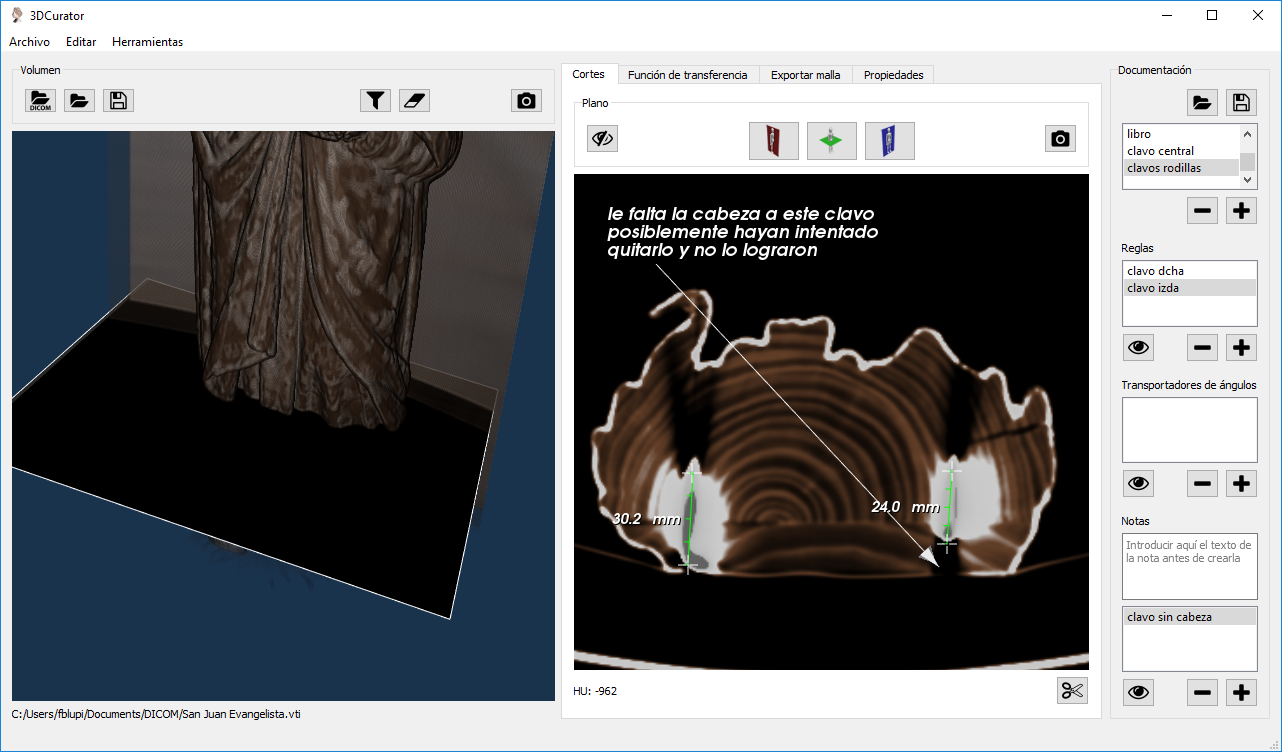
\includegraphics[width=12.5cm]{imagenes/resultados/documentacion/san-juan-evangelista/clavos-rodillas}
	\caption{Corte a la altura de las rodillas con la orientación adecuada para ver como hay otros dos clavos que unen las dos piezas del embón}
	\label{fig:resultados/documentacion/san-juan-evangelista/clavos-rodillas}
\end{figure}

Más abajo llegamos ya a la zona de los pies donde se ven otras dos varillas perpendiculares al resto que hemos visto hasta ahora (Figura \ref{fig:resultados/documentacion/san-juan-evangelista/varillas}). 

\begin{figure}[H]
	\centering
	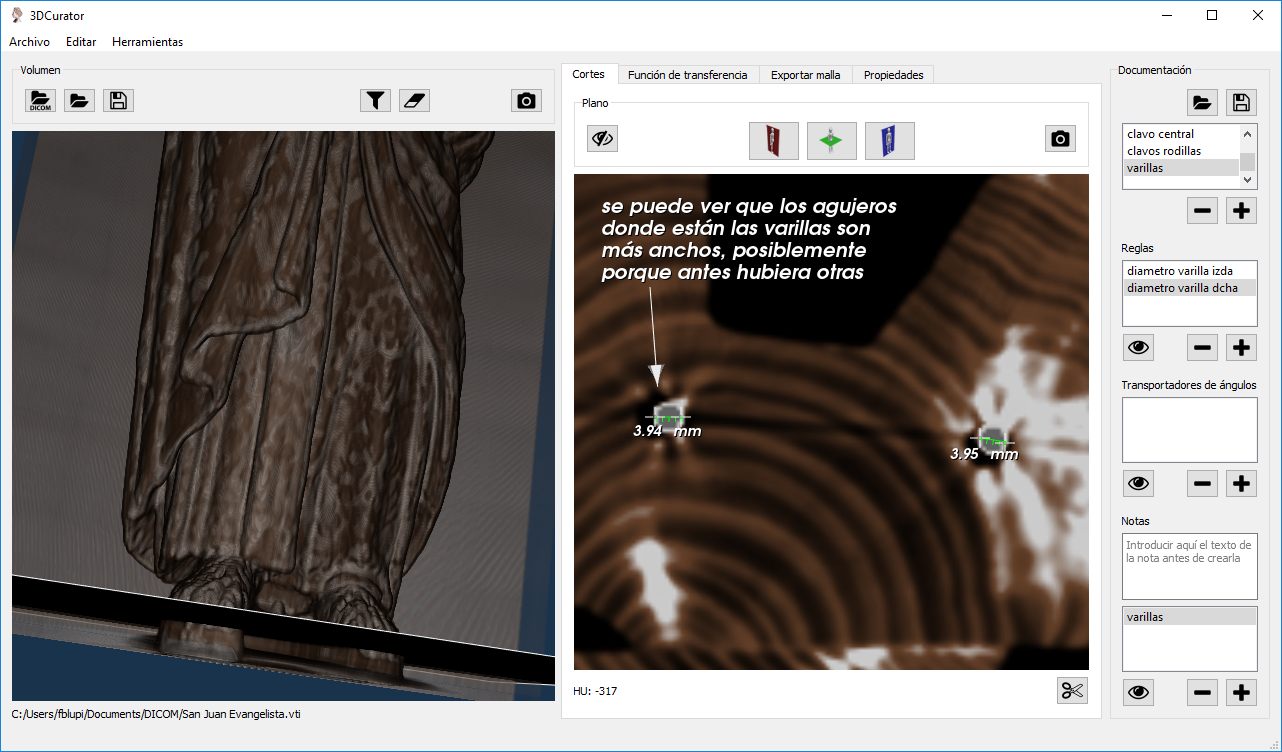
\includegraphics[width=12.5cm]{imagenes/resultados/documentacion/san-juan-evangelista/varillas}
	\caption{Corte axial a la altura de los gemelos donde se observan dos varillas de metal}
	\label{fig:resultados/documentacion/san-juan-evangelista/varillas}
\end{figure} 

El agujero de estas dos varillas puede ser que se hiciera antes y las varillas las colocarían al restaurarlas. 

Estas varillas forman parte de una plancha de hierro que produce mucho ruido (Figura \ref{fig:resultados/documentacion/san-juan-evangelista/varillas-coronal}). 

\begin{figure}[H]
	\centering
	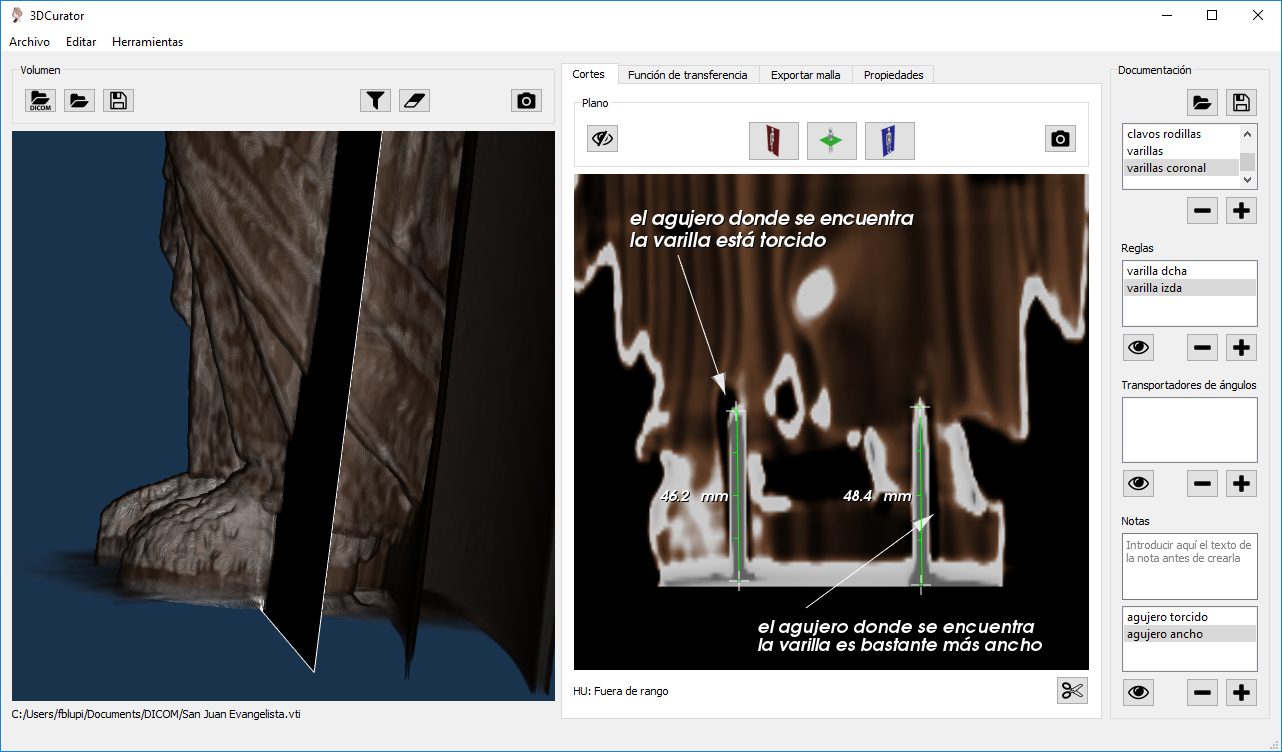
\includegraphics[width=12.5cm]{imagenes/resultados/documentacion/san-juan-evangelista/varillas-coronal}
	\caption{Corte coronal para estudiar la plancha de hierro de la base y las dos varillas que la unen a la figura}
	\label{fig:resultados/documentacion/san-juan-evangelista/varillas-coronal}
\end{figure} 
